

\mypart{Молитвы на разные случаи семейной жизни}
%http://www.molitvoslov.com/content/semeynoy-zhizni

 

\mychapter{Благословление на вступление в брак}
%http://www.molitvoslov.com/content/blagoslovenie-na-vstuplenie-vbrak

 

\section{Пресвятой Богородице в честь Ее иконы «Казанская»}
%http://www.molitvoslov.com/text9.htm 
 
\myfig{img/684.jpg}

\itshape Тропарь, глас 4-й:\normalfont{} Заступнице усердная, Мати Господа Вышняго! За всех молиши Сына Твоего, Христа Бога нашего, и всем твориши спастися, в державный Твой покров прибегающим. Всех нас заступи, о. Госпоже, Царице и Владычице, иже в напастех и в скорбех и в болезнех, обремененных грехи многими, предстоящих и молящихся Тебе умиленною душею и сокрушенным сердцем пред Пречистым Твоим образом со слезами, и невозвратно надежду имущих на Тя избавления всех зол. Всем полезная даруй и вся спаси, Богородице Дево: Ты бо еси Божественный покров рабом Твоим. 

\itshape 

Кондак, глас 8-й:\normalfont{} Притецем, людие, к тихому сему и доброму пристанищу, скорой Помощнице, готовому и теплому спасению, покрову Девы; ускорим на молитву и потщимся на покаяние: источает бо нам неоскудныя милости Пречистая Богородица, предваряет на помощь и избавляет от великих бед и зол благонравныя и богобоящияся рабы Своя. 

\itshape Молитва:\normalfont{} О Пречистая Владычице Богородице, Царице небеси и земли, вышшая ангел и архангел и всея твари честнейшая, чистая Дево Марие, миру благая помощнице и всем людем утверждение и во всяких нуждах избавление! Призри и ныне, Госпоже Всемилостивая, на рабы Твоя, Тебе умиленною душею и сокрушенным сердцем молящияся, со слезами к Тебе припадающия пречистому и цельбоносному образу Твоему, и помощи и заступления Твоего просящия. О Всемилостивая и Премилосердая Дево Богородице чтимая! Воззри, Госпоже, на люди Твоя: мы бо, грешнии, не имамы иныя помощи, разве Тебе и от Тебя рождшагося Христа Бога нашего. Ты еси заступница и предстательница наша, Ты еси обидимым защищение. Скорбящим радование, сирым прибежище, вдовам хранительница, девам слава, плачущим веселие, больным посещение, немощным исцеление, грешным спасение. Сего ради, о Богомати, к Тебе прибегаем и на Твой пречистый образ с превечным на руку Твоею держимым младенцем, Господем нашим Иисусом Христом взирающе, умиленное пение Тебе приносим и вопием: помилуй нас, Мати Божия, и прошение наше исполни, вся бо суть возможна ходатайству Твоему: яко Тебе слава подобает ныне и присно и во веки веков. Аминь.





\section{Благоверному князю Петру и княгине Февронии, Муромским чудотворцам}
%http://www.molitvoslov.com/text14.htm 
 
\myfig{img/685.jpg}

\itshape Молитва:\normalfont{} О велиции угодницы Божии и предивнии чудотворцы, благовернии княже Петре и княгине Февроние, града Мурома предстателие и хранителие, и о всех нас усерднии ко Господу молитвенницы! К вам прибегаем и вам с упованием крепким молимся: вознесите о нас, грешных, святыя молитвы ваша ко Господу Богу, и испросите у благости Его вся благопотребная душам и телесем нашим: веру праву, надежду благу, любовь нелицемерну, благочестие непоколебимо, в добрых делех преуспеяние, мира умирение, земли плодоносие, воздуха благорастворение, телесем здравие и душам спасение. Исходатайствуйте у Царя Небеснаго Церкви Святей и всей державе Российстей мир, тишину и благоустроение, и всем нам житие благополучное и добрую христианскую кончину. Оградите Отечество ваше и вся грады Российския от всякаго зла; и вся правоверныя люди, к вам приходящия и святым мощем вашим поклоняющиеся, осените благодатным действом богоприятных молитв ваших, и вся прошения их во благо исполните. Ей, чудотворцы святии! Не презрите молитв наших, со умилением вам днесь возносимых, но будите о нас приснии предстателие ко Господу, и сподобите нас помощию вашею спасение вечное улучити и Царствие Небесное унаследовати: да славословим неизреченное человеколюбие Отца и Сына и Святаго Духа, в Троице покланяемаго Бога, во веки веков. Аминь.


\bigskip\bigskip\mychapterending

\mychapter{О покровительстве вступающим в брак}
%http://www.molitvoslov.com/content/opokrovitelstve

 

\section{Святым бессребреникам и чудотворцам Косме и Дамиану}
%http://www.molitvoslov.com/text16.htm 
 
\bfseries Молитва:\normalfont{}


К вам, святии безсребренницы и чудотворцы Космо и Дамиане, яко к скорым помощником и теплым молитвенником о спасении нашем мы, недостойнии, преклонше колена, прибегаем и припадающе усердно вопием: не презрите моления нас грешных, немощных, во многая беззакония впадших, и по вся дни и часы согрешающих. Умолите Господа, да прибавит нам, недостойным рабом Своим, великия и богатыя Своя милости: избавите нас от всякия скорби и болезни, вы бо прияли есте от Бога и Спаса нашего Иисуса Христа неоскудную благодать исцелений, ради твердыя веры, безмезднаго врачевания и мученическия кончины вашея... Ей, угодницы Божии, не престайте молящеся за ны, с верою к вам притекающия: аще бо по множеству грехов наших и несмы достойни милосердия вашего, обаче вы вернии подражателие человеколюбия Божия суще, сотворите молитвами вашими, да плоды достойны покаяния приносяще, и в вечный покой достигнем, хваляще и благословяще дивнаго во святых Своих Господа и Бога и Спаса нашего Иисуса Христа, и Пречистую Матерь Его, и ваше теплое заступление всегда, ныне и присно и во веки веков. Аминь. 

 



\section{Молитва супругов при бракосочетании}
%http://www.molitvoslov.com/text890.htm 
 
\myfig{img/778.jpg}

Господи Боже наш, во спасительном Твоем смотрении сподобивый в Кане Галилей стей честный показати брак Твоим пришествием, Сам ныне рабы Тво\itshape я (имен\normalfont{}а) яже благоволил еси сочетатися друг другу, в мире и единомыслии сохрани; честный их брак покажи, нескверное их ложе соблюди, непорочное их сожительство пребывати благослови и сподобия к старости маститей достигнути, чистым сердцем делающе заповеди Твоя. Ты бо еси Бог наш, Бог еже миловати и спасати, и Тебе славу воссылаем, со Безначальным Твоим Отцем, Всесвятым и Благим и Животворящим Твоим Духом, ныне и присно и во веки веков. Аминь. 





\section{Молитва о семье}
%http://www.molitvoslov.com/text937.htm 
 
\myfig{img/870.jpg}

«Не бойся, малое стадо! Аз есмь с вами и никтоже на вы».


Владычице Преблагословенная, возьми под Свой покров семью мою. Всели в сердца супруга моего и чад наших мир, любовь и непрекословие всему доброму;  не допусти никого из семьи моей до разлуки и тяжкаго расставания, до преждевременныя и внезапныя смерти без покаяния.

А дом наш и всех нас, живущих в нем, сохрани от огненнаго запаления, воровскаго нападения, всякаго злаго обстояния, разнаго страхования и диавольскаго наваждения.

Да и мы купно и раздельно, явно и сокровенно будем прославлять имя Твое Святое всегда, ныне и присно, и во веки веков. Аминь.


Пресвятая Богородице, спаси нас!


\bigskip\bigskip\mychapterending

\mychapter{О счастии брака}
%http://www.molitvoslov.com/content/oschastiibraka

 

%~ \section{Пресвятой Владычице нашей Богородице и Приснодеве Марии}
%http://www.molitvoslov.com/text18.htm 
{\noparindent\begin{minipage}{\textwidth}
\myfig{img/10_0.jpg}\section{Пресвятой Владычице нашей Богородице и Приснодеве Марии}
\restoreparindent
\bfseries Тропарь, глас 4-й:\normalfont{}

%\twocolumns{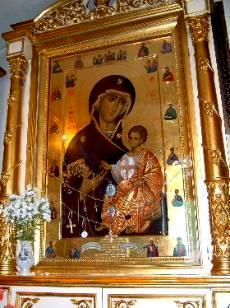
\includegraphics[width=\linewidth]{img/10_0.jpg}}{
%\setlength\parindent{\myparindent}
%\bfseries Тропарь, глас 4-й:\normalfont{}

Рождество Твое, Богородице Дево, радость возвести всей вселенней: из Тебе бо возсия Солнце правды Христос Бог наш, и разрушив клятву, даде благословение, и упразднив смерть, дарова нам живот вечный.


\medskip


\bfseries Кондак, глас 4-й:\normalfont{}


Иоаким и Анна поношения безчадства, и Адам и Ева от тли смертныя свободистася, Пречистая, во святем Рождестве Твоем. То празднуют и людие Твои, вины прегрешений избавльшеся, внегда звати Ти: неплоды раждает Богородицу и Питательницу жизни нашея.

\end{minipage}}

{\bigskip\bigskip\noparindent\begin{minipage}{\textwidth}
\myfigr[0.3]{img/12_0.jpg}\section{Архангелу Варахиилу "--- покровителю благочестивых семейств, Небесным чинам бесплотным}
%http://www.molitvoslov.com/text19.htm 

\restoreparindent\bfseries Молитва:\normalfont{}\par

О великий архистратиже Божий архангеле Варахииле! Предстоя Престолу Божию и оттоли принося благословения Божия в домы верных раб Божиих, испроси у Господа Бога милосердия и благословения на домы наша, да благословит Господь Бог нас и умножит изобилие плодов земных, и подаст нам здравие и спасение, во всем благое поспешение, и на врагов победу и одоление, и сохранит нас на многая лета, всегда. Ныне и присно и во веки веков. Аминь.
\end{minipage}}

\section{Молитва апостолу Симону Зилоту}
%http://www.molitvoslov.com/text20.htm 
 
\myfig[0.33]{img/11_1.jpg}\bfseries Кондак, глас 2-й:\normalfont{}


Известно премудрости учения в душах благочествующих положшаго во хвалении ублажим, яко Богоглаголиваго вси Симона: Престолу бо Славы ныне предстоит и со Безплотными веселится, моляся непрестанно о всех нас.


\medskip
\bfseries Молитва:\normalfont{}


Святый славный и всехвальный апостоле Христов Симоне, сподобивыйся прияти в дом твой в Кане Галилейстей Господа нашего Иисуса Христа и Его Пречистую Матерь, Владычицу нашу Богородицу, и очевидцем быти преславнаго чудесе Христова, на браце твоем явленного, претворения воды в вино! Молим тя с верою и любовшо: умоли Христа Господа претворить души наша из грехолюбивых в боголюбивыя; сохрани и соблюди нас молитвами твоими от искушений диавольских и падений греховных и испроси нам свыше помощь во время уныния и беспомощия нашего, да не преткнемся о камень соблазна, но неуклонно шествуем спасительным путем заповедей Христовых, дондеже достигнем обителей райских, идеже ты ныне водворяешися и веселишися. Ей, апостоле Спасов! Не посрами нас, крепце на тя уповающих, но буди нам помощник и покровитель во всем житии нашем и помози нам благочестно и богоугодно житие сие временное скончати, благую и мирную христианскую кончину получити и добраго ответа сподобитися на Страшнем Суде Христове, да избежавше мытарств воздушных и власти лютаго миродержца, унаследуем Царство Небесное и прославим великолепое Имя Отца и Сына и Святаго Духа во веки веков. Аминь.

\bigskip\bigskip\mychapterending

\mychapter{О совете и любви между мужем и женой}
%http://www.molitvoslov.com/content/osoveteilubvi

 
\vspace{-\baselineskip}{\noparindent\begin{minipage}{\textwidth}
\myfig[0.29]{img/13_0.jpg}\section{Святому апостолу и евангелисту Иоанну Богослову}
%http://www.molitvoslov.com/text22.htm 

\restoreparindent\bfseries Молитва:\normalfont{}

О великий и всехвальный апостоле и евангелисте Иоанне Богослове, наперсниче Христов, теплый наш заступниче и скорый в скорбех помощниче! Умоли Господа Бога даровати нам оставление всех прегрешений наших, елико согрешихом от юности нашея, во всем житии нашем, делом, словом, помышлением и всеми нашими чувствы. Во исходе же душ наших помози нам, грешным, избавитися воздушных мытарств и вечнаго мучения, да твоим милостивным предстательством прославляем Отца и Сына и Святаго Духа, ныне и присно и во веки веков. Аминь.
\end{minipage}}

\longpage{}

{\bigskip\noparindent\begin{minipage}{\textwidth}
\myfigr[0.26]{img/381_0.jpg}\section{Благоверному князю Даниилу Московскому}
%http://www.molitvoslov.com/text516.htm 
 
\restoreparindent\bfseries Молитва:\normalfont{}

Церкве Христовы похвало высокая, града Москвы стено необоримая, державы Российския Божественное утверждение, преподобне княже Данииле, к раце мощей твоих притекающе, усердно молим тя: призри на нас, память твою воспевающих, пролей теплое твое ходатайство ко Спасу всех, яко да утвердит миром страну нашу, грады и веси ея и обитель сию добре да сохранит, благочестие и любовь в людях твоих насаждая, злобу же, междоусобие и нравов развращение искореняя; всем же нам вся благая ко временному животу и вечному спасению даруй молитвами твоими, яко да прославляем дивного во святых Своих Христа Бога нашего во веки веков. Аминь.
\end{minipage}}

\mychapterending

\mychapter{О всякой семейной и бытовой нужде}
%http://www.molitvoslov.com/content/ovsyakoynuzhde

 

\section{Святой блаженной Ксении Петербургской}
%http://www.molitvoslov.com/text623.htm 
 
\bfseries Тропарь, глас 7-й:\normalfont{}


Нищету Христову возлюбивши, безсмертныя трапезы ныне наслаждаешися, безумием мнимым безумие мира обличивши, смирением крестным силу Божию восприяла еси. Сего ради дар чудодейственныя помощи стяжавшая, Ксение блаженная, моли Христа Бога избавитися нам от всякого зла покаянием.


\medskip
\bfseries Кондак, глас 3-й:\normalfont{}


Днесь светло ликует град святого Петра, яко множество скорбящих обретают утешение, на твоя молитвы надеющеся, Ксение всеблаженная, ты бо еси граду сему похвала и утверждение.


\medskip
\bfseries Молитва:\normalfont{}


О, святая всеблаженная мати Ксение! Под кровом Всевышняго жившая, ведомая и укрепляемая Богоматерию, глад и жажду, хлад и зной, поношения и гонения претерпевшая, дар прозорливости и чудотворения от Бога прияла еси и под сению Всемогущего покоишися. Ныне Святая Церковь, яко благоуханный цвет, прославляет тя: предстояще на месте погребения твоего, пред образом твоим святым, яко живей ти, сушей с нами, молимся ти: приими прошения наша и принеси их ко Престолу Милосердаго Отца Небеснаго, яко дерзновение к Нему имущая, испроси притекающим к тебе вечное спасение, и на благая дела и начинания наша щедрое благословение, от всяких бед и скорбей избавление, предстани святыми твоими молитвами пред Всемилостивым Спасителем нашим о нас, недостойных и грешных, помози, святая блаженная мати Ксение, младенцы светом Святаго Крещения озарити и печатию дара Духа Святаго запечатлети, отроки и отроковицы в вере, честности, богобоязненности и целомудрии воспитати и успехи в учении им даровати; болящия и недугующия исцели, семейным любовь и согласие низпосли, монашествующим подвигом добрым подвизатися удостой и от поношений огради, пастыри в крепости духа утверди, народ и страну нашу в мире и безмятежии сохрани, о лишенных в предсмертный час причащения Святых Христовых Тайн умоли: ты наша надежда и упование, скорое услышание и избавление, тебе благодарение возсылаем и с тобою славим Отца и Сына и Святаго Духа, ныне и присно и во веки веков. Аминь.

\section{Святой блаженной Ксении Петербургской}
%http://www.molitvoslov.com/text25.htm 
 
\myfig{img/15_0.jpg}\bfseries Молитва:\normalfont{}


О, препростая образом жития своего, бездомная на земли, наследнице же обителей Отца Небеснаго, блаженная страннице Ксение! Якоже прежде к надгробию твоему недужнии и скорбнии припадавшии и абие утешениями исполняемии, сице ныне и мы, обуреваемии тлетворными обстоянии, к тебе прибегающе, с надеждою просим: помолися, благая небошественнице, дабы исправилися стопы наша по словеси Господню к деланию заповедей Его, и да упразднится богоборное безбожие, пленившее град твой и страну твою, привергающее нас многогрешных в смертное братоненавидение, гордое самовозбешение и хульное отчаяние. О, блаженнейшая Христа ради, посрамившая суемудрость века сего, испроси у Творца и Подателя всяческих благ даровати нам смирения, кротости и любве в сокровище сердца нашего, веры в укрепление молитвы, надежды в покаянии, крепости в многотрудном житии, милосерднаго исцеления души и тела нашего, целомудрия в супружестве и благопопечения о ближних и искренних своих, всего жития нашего обновление в чистительней бане покаяния, яко да всехвально воспевающе память твою, прославим, в тебе чудодействующаго, Отца и Сына и Святаго Духа, Троицу Единосущную и Нераздельную во веки веков. Аминь.

\bigskip\bigskip\mychapterending

\mychapter{При детородном неплодстве}
%http://www.molitvoslov.com/content/pri-detorodnom-neplodstve

 

\section{Святому пророку Захарии и Елисавете}
%http://www.molitvoslov.com/text30.htm 
 
\bfseries Тропарь:\normalfont{}


Священства одеждою обложен, премудре, по Закону Божию всесожжения приятна священнолепно приносил еси, Захарие, и был еси светильник и зритель тайных, знамения в тебе благодати нося явственно, всемудре. И мечем убиен был в храме Божии, Христов пророче, с Предтечею моли спастися душам нашим.


\medskip
\bfseries Иной тропарь:\normalfont{}


Праведных Твоих Захарии и Елисаветы, Господи, память празднующе, теми молим Тя: спаси души наша.


\medskip
\bfseries Кондак:\normalfont{}


Пророк днесь и священник Вышняго, Захария предложи, Предтечев родитель, трапезу своея памяти, верныя питая, питие бо правды всем растворив, сего ради скончавается, яко Божественный таинник Божия благодати.


\medskip
\bfseries Молитва:\normalfont{}


О святии угодницы Божии, пророче Захарие и праведная Елисавето! Подвигом добрым подвизавшеся на земли, восприяли есте на небесех венец правды, егоже уготовал есть Господь всем любящим Его. Темже взирающе на святый ваш образ, радуемся о преславнем скончании жительства вашего и чтим святую память вашу. Вы же, предстоя Престолу Божию, приимите моления наша и ко Всемилостивому Богу принесите, о еже простити нам всякое прегрешение и помощи нам стати противу кознем диавольским, да избавльшеся от скорбей, болезней, бед и напастей и всякаго зла, благочестно и праведно поживем в нынешнем веце и сподобимся предстательством вашим, аще и недостойни есмы, видети благая на земли живых, славяще Единаго во святых Своих славимаго Бога, Отца и Сына и Святаго Духа, ныне и во веки веков. Аминь.

\newpage\section{Праведным богоотцам Иоакиму и Анне}
%http://www.molitvoslov.com/text27.htm 
 
\myfig{img/16.jpg}\bfseries Тропарь, глас 1-й:\normalfont{}


Иже в законней благодати праведни бывше, Младенца Богоданного породиша нам, Иоаким и Анна. Темже днесь светло торжествует, весело празднующи Божественная Церковь, честную вашу память, славящи Бога, воздвигшаго рог спасения нам в дому Давидове.


\medskip
\bfseries Кондак, глас 2-й:\normalfont{}


Радуется ныне Анна. Неплодства разрешившися соуз, и питает Пречистую, созывающи вся воспети Даровавшаго от чрева ея человеком, Едину Матерь и Неискусомужную.


\medskip
\bfseries Молитва:\normalfont{}


О, приснославнии Христовы праведницы, святии богоотцы Иоакиме и Анно, предстоящии Небесному Престолу Великого Царя и велие дерзновение к Нему имущии, яко от Преблагословенныя Дщере вашея, Пречистыя Богородицы и Приснодевы Марии, воплотитися изволившему!

К вам, яко многомощным предстателем и усердным о нас молитвенником, прибегаем мы, грешнии и недостойнии. Молите благость Его, яко да отвратит от нас гнев Свой, по делом нашим праведно на ны движимый, и да безчисленная прегрешения наша презрев, обратит нас на путь покаяния, и на стези заповедей Своих да утвердит нас. Также молитвами вашими в мире жизнь нашу сохраните, и во всех благих благое поспешение испросите, вся к животу и благочестию потребная нам от Бога дарующи, от всяких напастей и бед и внезапные смерти предстательством вашим нас избавляюще, и от всех враг видимых и невидимых защищающе, яко да тихое и безмолвное житие поживем во всяком благочестии и чистоте, и такое в мире временное сие житие прешедше, в вечный достигнем покой, идеже вашим святым умолением да сподобимся Небеснаго Царствия Христа Бога нашего, Емуже, со Отцем и Пресвятым Духом, подобает всякая слава, честь и поклонение во веки веков. Аминь.

\section{Молитва супругов о даровании детей}
%http://www.molitvoslov.com/text29.htm 
 


Услыши нас, Милосердный и Всемогущий Боже, да молением нашим ниспослана будет благодать Твоя. Будь милостив, Господи, к молитве нашей, вспомни Закон Твой об умножении рода человеческаго и буди милостивым Покровителем, да Твоею помощию сохранится Тобою же установленное. Ты властною силою Твоею из ничего все сотворил и положил начало всего в мире существующего "--- сотворил и человека по образу Своему и высокою тайною освятил союз супружества и предуказание тайны единения Христа с Церковью. Призри, Милосердный, на рабов Твоих сих (имена), союзом супружеским соединенных и умоляющих о Твоей помощи, да будет на них милость Твоя, да будут плодовиты и да увидят они сына сынов своих даже до третьяго и четвертаго рода и до желаемой старости доживут и войдут в Царство Небесное через Господа нашего Иисуса Христа, Которому всякая слава, честь и поклонение подобает со Святым Духом во веки. 


\section{Преподобному Роману}
%http://www.molitvoslov.com/text517.htm 
 
\bfseries Тропарь, глас 8 -й:\normalfont{}


В тебе, отче, известно спасеся еже по образу: приим бо крест последовал еси Христу,  и дея учил еси презирати убо плоть, приходит бo, прилежати же о души, вещи безсмертней. Tем же и со aнгелы срадуется, преподобне Романе, дух твой.


Чистотою душевною Божественно вооружився, и непристанныя молитвы яко копие вручив крепко, пробол еси бесовская ополчения, Романе отче наш, моли непрестанно о всех нас.


\medskip
\bfseries Молитва:\normalfont{}


О священная главо, преподобне отче, преблаженне авво Романе, не забуди убогих твоих до конца, но поминай нас всегда во святых и благоприятных молитвах к Богу: помяни стадо твое, еже сам упасл еси, и не забуди посещати чад твоих. Mоли за ны, отче священный, за дети твоя духовныя, яко имеяй дерзновение к Небесному Царю: не премолчи за ны ко Господу, и не презри нас, верою и любовию чтущих тя: поминай нас недостойных у Престола Вседержителева, и не престай молитися о нас ко Христу Богу, ибо дана тебе бысть благодать за ны молитися. Не мним бо тя суща мертва: аще бо телом и преставился еси от нас, но и по смерти жив сый пребываеши, не отступай от нас духом, сохраняя нас от стрел вражиих и всякия прелести бесовския и козней диавольских, пастырю наш добрый аще бо и мощей твоих рака пред очима нашима видима есть всегда, но святая твоя душа со ангельскими воинствы, со Безплотными лики, с Небесными Силами, у Престола Вседержителева предстояши, достойно веселится, ведуще убо тя воистину и по смерти жива суща, тебе припадаем и тебе молимся: молися о нас Всесильному Богу, о пользе душ наших, и испроси нам время на покаяние, да невозбранно прейдем от земли на небо, от мытарств же горьких, бесов воздушных князей и от вечныя муки да избавимся, и Небеснаго Царствия наследницы да будем со всеми праведными, от века угодившими Господу нашему Иисусу Христу: Ему же подобает всякая слава, честь и поклонение, со Безначальным Его Отцем, и с Пресвятым и Благим и Животворящим Его Духом, ныне и присно, и во веки веков. Аминь.


\medskip
\bfseries Величание:\normalfont{}


Ублажаем тя, преподобне отче Романе, и чтим святую память твою, наставниче монахов и собеседниче aнгелов.

\longpage[2]{}\mychapterending

\mychapter{При желании иметь дитя мужского пола}
%http://www.molitvoslov.com/content/imet-ditya-muzhskogo-pola

 

\section{Преподобному Александру Свирскому}
%http://www.molitvoslov.com/text38.htm 
 
\myfig{img/24.jpg}\bfseries Молитва:\normalfont{}


О, священная главо, ангеле земный и человече небесный, преподобне и богоносне отче наш Александре, изрядный угодниче Пресвятыя и Единосущныя Троицы, многия милости живущим во святей обители твоей и всем, с верою и любовию притекающим к тебе, являяй. Испроси нам вся к житию сему временному благопотребная, паче же к вечному спасению нашему нужная. Пособствуй предстательством твоим, угодниче Божий, правителем страны нашея России. И да в мире глубоце пребудет святая православная Церковь Христова. Буди всем нам, чудотворче святый, во всякой скорби и обстоянии скорый помощниче. Наипаче же в час кончины нашея явися нам, заступниче благосердый, да не предани будем на мытарствах воздушных власти злобнаго миродержца, но да сподобимся непреткновеннаго восхода в Царствие Небесное. Ей, отче, молитвенниче наш присный! Не посрами упования нашего, не презри смиренных молений наших, но присно о нас пред Престолом Живоначальныя Троицы предстательствуй, да сподобимся вкупе с тобою и со всеми святыми, аще и недостойны есмы, в селениих райских славити величие, благодать и милость Единаго в Троице Бога, Отца и Сына и Святаго Духа во веки веков. Аминь.

\bigskip\bigskip\mychapterending

\mychapter{Молитвы беременных женщин о благополучном разрешении и о рождении здоровых детей}
%http://www.molitvoslov.com/content/molitv-beremennih-zhenchin

 

\section{Пресвятой Богородице перед Ее иконой «Целительница»}
%http://www.molitvoslov.com/text42.htm 
 
\myfig{img/26_0.jpg}

\bfseries Тропарь, глас 4-й:\normalfont{}


Яко Пресветлая Звездо, просия Божественными чудесы святый Твой образ Целительнице. Подаждь убо и нам, Богородице Марие, исцеление недугов душевных и телесных, спасение и велию милость.


\medskip


\bfseries Молитва:\normalfont{}


Приими, о, Всеблагословенная и Всемощная Госпоже Владычице Богородице Дево, сия молитвы, со слезами Тебе ныне приносимыя от нас, недостойных раб Твоих, ко Твоему цельбоносному образу пение возсылающих со умилением, яко Тебе Самой зде сущей и внемлющей молению нашему. По коемуждо бо прошению исполнение твориши, скорби облегчаеши, немощным здравие даруеши, разслабленныя и недужныя исцеляеши, от бесных бесы прогоняеши, обидимыя от обид избавлявши, прокаженныя очищаеши и малыя дети милуеши; еще же, Госпоже Владычице Богородице, и от уз и темниц свобождаеши и всякия многоразличныя страсти врачуеши: вся бо суть возможна ходатайством Твоим к Сыну Твоему, Христу Богу нашему. О, Всепетая Мати, Пресвятая Богородице! Не престай молитися о нас недостойных рабах Твоих, славящих Тя и почитающих Тя, и поклоняющихся со умилением Пречистому образу Твоему, и надежду имущих невозвратну и веру несумненну к Тебе, Приснодеве Преславней и Непорочней, ныне и присно и во веки веков. Аминь.


\section{Пресвятой Богородице перед Ее иконой «Скоропослушница»}
%http://www.molitvoslov.com/text40.htm 
 
\bfseries Тропарь, глас 4-й:\normalfont{}
К Богородице притецем сущии в бедах, и святей иконе Ея ныне припадем, с верою зовуще из глубины души: скоро наше услыши моление, Дево, яко Скоропослушница нарекшаяся, Тебе бо ради раби Твои в нужду готовую помощницу имамы.


\medskip
\bfseries Кондак, глас 8-й:\normalfont{}


В мори житейстем обуреваемии, треволнению подпадаем страстей и искушений. Подаждь убо нам, Госпоже, руку помощи, якоже Петрови Сын Твой, и ускори от бед избавити ны, да зовем Ти: радуйся, всеблагая Скоропослушнице.


\medskip
\bfseries Молитва:\normalfont{}


Преблагословенная Владычице, Приснодево Богородице, Бога Слова паче всякаго слова на спасение наше рождшая, и благодать Его преизобильно паче всех приявшая, море явльшаяся Божественных дарований и чудес приснотекущая река, изливающая благость всем, с верою к Тебе прибегающим! Чудотворному Твоему образу припадающе, молимся Тебе, всещедрей Матери человеколюбиваго Владыки: удиви на нас пребогатыя милости Твоя и прошения наша, приносимая Тебе, Скоропослушнице, ускори исполнити все, еже на пользу во утешение и спасение коемуждо устрояющи. Посети, Преблагая, рабы Твоя благодатию Твоей, подаждь недугующим цельбу и совершенное здравие, обуреваемым тишину, плененным свободу, и различными образы страждущих утеши. Избави, Всемилостивая Госпоже, всяк град и страну от глада, язвы, труса, потопа, огня, меча и иныя казни временныя и вечныя, Матерним Твоим дерзновением отвращающи гнев Божий; и душевнаго разслабления, обуревания страстей и грехопадений свободи рабы Твоя, яко да непреткновенно во всяком благочестии поживше в сем веце, и в будущем вечных благ сподобимся благодатию и человеколюбием Сына Твоего и Бога, Емуже подобает всякая слава, честь и поклонение со Безначальным Его Отцем и Пресвятым Духом, ныне и присно и во веки веков. Аминь.

При недостатке молока также молятся пред иконой Пресвятой Богородицы «Скоропослушница».

\section{Преподобной Мелании Римляныне}
%http://www.molitvoslov.com/text45.htm 
 
\bfseries Тропарь:\normalfont{}


В тебе, мати, известно спасеся, еже по образу: приимши бо крест, последовала еси Христу, и деющи учила еси презирати убо плоть, преходит бо; прилежати же о души, вещи безсмертней; темже и со ангелы срадуется, преподобная Мелание, дух твой.


\medskip
\bfseries Кондак, глас 3-й:\normalfont{}


Девства чистоты возлюбши, и обручника к благим увещавши, премножество богатства расточи в пребывание иночествующим, богоблаженная, и обители воздвиже. Темже в небесная обители вселися, поминай нас, Мелание всечестная.

Также при беременности и трудных родах молятся перед Албазинской иконой Божией Матери «Слово плоть бысть» и перед иконой «Помогательница женам чады раждати».

\section{Молитва беременных женщин о благополучном разрешении}
%http://www.molitvoslov.com/text44.htm 
 


О, Преславная Матерь Божия, помилуй меня, рабу Твою, и прииди ко мне на помощь во время моих болезней и опасностей, с которыми рождают чад все бедные дщери Евы. Вспомни, о Благословенная в женах, с какою радостию и любовию Ты шла поспешно в горнюю страну посетить сродницу Твою Елисавету во время ея беременности и какое чудесное действие произвело благодатное посещение Твое и в матери, и в младенце. И по неисчерпаемому благосердию Твоему даруй и мне, уничиженней рабе Твоей, разрешитися от бремени благополучно; даруй мне сию благодать, чтобы дитя, покоящееся теперь под моим сердцем, пришедши в чувство, с радостным взыгранием, подобно святому младенцу Иоанну, поклонялось Божественному Господу Спасителю, Который из любви к нам, грешным, не возгнушался и Сам стать Младенцем. Неизглаголанная радость, которою преисполнилось девственное Твое сердце при воззрении на новорожденного Твоего Сына и Господа, да усладит скорбь, предстоящую мне среди болезней рождения. Жизнь мира, мой Спаситель, рожденный Тобою, да спасет меня от смерти, пресекающей жизнь многих матерей в час разрешения и да причтет плод чрева моего к числу избранных Божиих. Услыши, Пресвятая Царице Небесная, смиренную мольбу мою и призри на меня, бедную грешницу, оком Твоея благодати; не постыди моего упования на Твое великое милосердие и осени меня. Помощница христиан, Исцелительница болезней, да сподоблюсь и я испытать на себе, что Ты "--- Матерь милосердия, и да прославлю всегда Твою благодать, не отвергшую никогда молитвы бедных и избавляющую всех призывающих Тебя во время скорби и болезней. Аминь. 


\newpage\section{Пресвятой Богородице перед Ее иконой «Феодоровская»}
%http://www.molitvoslov.com/text43.htm 
 
\myfig{img/27_0.jpg}\bfseries Тропарь,глас 4-й:\normalfont{}


Пришествием честныя Твоея иконы, Богоотроковице, обрадованный днесь, богохранимый град Кострома, якоже древний Израиль к кивоту завета, притекает ко изображению лица Твоего и воплотившагося от Тебе Бога нашего, да Твоим Матерним к нему предстательством присно ходатайствуеши всем под сень крова Твоего прибегающим мир и велию милость.


\medskip
\bfseries Кондак 1-й:\normalfont{}


Взбранней Воеводе, Пренепорочней Деве Богородице, Заступнице нашей и Предстательству христиан непостыдному, явлением чудныя иконы Своея радование подавшей земле Российстей и вся верныя чада Церкве просветившей, благодарение усердно приносим Ти, Богородице, и припадающе пречудному образу Твоему, умильно глаголем. Спаси, Госпоже, и помилуй рабы Твоя, зовущия: Радуйся, Матерь Божия, Предстательнице и Заступнице наша усердная.


\medskip
\bfseries Молитва:\normalfont{}


К кому воззову, Владычице, к кому прибегну в печали моей; к кому принесу слезы и воздыхания моя, аще не к Тебе, Царице Небеси и земли: кто исторгнет мя от тины грехов и беззаконий, аще не Ты, о Мати Живота, Заступнице и Прибежище рода человеческаго. Услыши стенание мое, утеши мя и помилуй в горести моей, защити в бедах и напастях, избави от озлоблений и скорбей, и всяких недугов, и болезней, от враг видимых и невидимых, умири вражду стужающих мне, да избавлен буду от клеветы и злобы человеческия; такожде от своея ми плоти гнусных обычаев свободи мя. Укрый мя под сению милости Твоея, да обрящу покой и радость и от грехов очищение. Твоему Матернему заступлению себе вручаю; буди мне Мати и надеждо, покров, и помощь, и заступление, радость и утешение, и скорая во всем Помощнице. О, чудная Владычице! Всяк притекает к Тебе, без Твоея всесильныя помощи не отходит; сего ради и аз недостойный к Тебе прибегаю, да избавлен буду от внезапныя и лютыя смерти, скрежета зубнаго и вечнаго мучения. Небесное же Царствие получити сподоблюся и Тебе во умилении сердца реку: Радуйся, Мати Божия, Предстательница и Заступница наша усердная, во веки веков. Аминь.

\bigskip\bigskip\mychapterending

\mychapter{О здравии младенцев}
%http://www.molitvoslov.com/content/ozdravii-mladencev

 

\section{Молитва поименованному отрочати}
%http://www.molitvoslov.com/text880.htm 
 


\itshape Молитвы читает священник\normalfont{}

Господи Боже наш, в четыредесятный день младенец законному храму принесенный от Марии неискусобрачныя и Святыя Твоея Матере, и на объятиях праведнаго Симеона носимый, Сам Владыко всесильне, и принесеннаго сего младенца, явитися Тебе всех Творцу, благослови и на всякое дело благое и Тебе благоугодное возрасти, отгоняя от него всякую сопротивную силу, знамением воображения Креста Твоего. Ты бо еси храняй младенцы, Господи; да сподобився святаго Крещения, получит часть избранных Царствия Твоего, соблюдаемь с нами благодатию Святыя и Единосущныя, и Нераздельныя Троицы: Тебе бо подобает всякая слава, благодарение, и поклонение со Безначальным Твоим Отцем, и Пресвятым, и Благим, и Животворящим Твоим Духом, ныне и присно и во веки веков. Аминь. 


Боже Отче Вседержителю, велегласней шим пророком Исаием предвозвестивый нам, еже от Девы воплощение Единороднаго Твоего Сына и Бога нашего, иже в последния дни благоволением Твоим, и содействием Святаго Духа, спасения ради нас человеков, безмерным благоутробием от Нея младенствовати изволивый, и по обычаю в законе святом  Твоем, по исполнении дней очищения, святилищу принестися претерпе истинный Законоположник Сый; и на объятиях праведнаго Симеона носитися изволи, егоже таинства проображение в предреченном пророце, клещами угля явленное познахом; егоже и мы вернии подражание благодатию держим. Сам и ныне, сохраняяй младенцы Господи, благослови отроча сие, вкупе с родители и восприемники его, и сподоби его во время благопотребное и водою и Духом отрождения, сопричти е Святому Твоему стаду словесных овец, нарицающихся именем Христа Твоего: яко Ты еси в вышних Живый, и на смиренныя призираяй, и Тебе славу возсылаем, Отцу, и Сыну, и Святому Духу, ныне и присно и во веки веков. Аминь.





\section{Молитва при наречении имени дитяти в восьмой день по его рождении}
%http://www.molitvoslov.com/text877.htm 
 


\itshape Молитвы читает священник\normalfont{}

Господи Боже наш, Тебе молимся, и Тебе просим, да знаменается свет Лица Твоего на рабе Твоем сем [на рабе Твоей сей]\itshape  (имя)\normalfont{}, и да знаменается Крест Единороднаго Сына Твоего в сердце и в помышлениях его, во еже бегати суеты мира, и от всякаго лукаваго навета вражия, последовати же повелени ем Твоим. Идаждь Господи, не отреченну пребыти имени Твоему святому на нем, совокупляемем во время благопотребно святей Твоей Церкви, и совершаемем страшными тайнами Христа Твоего; да по заповедем Твоим жительствовав, и сохранив печать нерушиму, получит блаженство избранных во Царствии Твоем, благодатию и человеколюбием Единороднаго Сына Твоего, с Ним же благословен еси, с Пресвятым, и Благим и Животворящим Твоим Духом, ныне и присно и во веки веков. Аминь. 


\section{Молитвы в первый день по рождению дитяти}
%http://www.molitvoslov.com/text876.htm 
 


\itshape Молитвы читает священник\normalfont{}

Владыко Господи Вседержителю, исцеляяй всякий недуг и всякую язву, сам и сию днесь родившую рабу Твою\itshape  (имя)\normalfont{}, исцели, и возстави ю от одра, на немже лежит: зане, по пророка Давида словеси, в беззакониих зачахомся, и сквернави вси есмы пред Тобою. Сохрани сию, и сего младенца, егоже роди: покрый ю под кровом крилу Твоею, от днешняго дне даже до последняго ея скончания, молитвами Пречистыя Богородицы и всех святых; яко благословен еси во веки веков, аминь. 


Владыко Господи Боже наш, родивыйся от Пречистыя Владычицы нашея Богороди цы и Приснодевы Марии, и яко младенец во яслех возлегий, и яко детищ восприемлем бывый; Сам и сию рабу Твою, днесь родившую сие отроча, помилуй, и прости вольныя и невольныя ея прегрешения, и сохрани ю от всякаго диавольскаго мучительства; и из нея рожденнаго младенца соблюди от всякаго яда, от всякия лютости, от всякия бури сопротивнаго, от духов лукавых, дневных же и нощных. Сию же соблюди под державною рукою Твоею, и даждь ей скорое востание, и от скверны очисти, и болезни исцели, и здравие и благомощие души же и телу даруй, и Ангелы светлыми и сияющими сию огради; и соблюди от всякаго наития невидимых духов. Ей Господи, от недуга и слабости, от ревности и зависти, и от очес призора, и помилуй ю и младенца, по велицей милости Твоей, и очисти ю от телесныя скверны, и различных ей находящих утробных стужений; и изведи ю скорою милостию Твоею во смиренном ея теле во исправление: и из нея рожденнаго младенца сподоби поклонитися земному храму, егоже уготовал еси славословитися имени Твоему святому. Яко подобает Тебе всякая слава, честь и поклонение, Отцу, и Сыну, и Святому Духу, ныне и присно и во веки веков. Аминь.  


Господи Боже наш, благоволивый снити с небес, и родитися от святыя Богородицы и Приснодевы Марии, спасения ради нас грешных, ведый немощное человеческаго естества, прости рабе Твоей \itshape (имя)\normalfont{}, днесь родившей, по множеству щедрот Твоих. Ты бо рекл еси Господи: раститеся и умножайтеся, и исполните землю и обладайте ею. Сего ради и мы, раби Твои, молимся, и дерзающе незлобивым Твоим человеколюбием, со страхом вопием к Царствия Твоего Святому имени: призри с небесе и виждь немощь нас осужденных, и прости рабе Твоей сей (\itshape имя\normalfont{}) , и всему дому, в немже родися отроча, и при коснувшымся ей, и зде обретающымся всем, яко Благ и Человеколюбец Бог прости: яко Един имаши власть оставляти грехи, молитвами Пречистыя Богородицы и всех святых Твоих. Аминь.





\section{Молитва святому праведному Симеону Богоприимцу}
%http://www.molitvoslov.com/text875.htm 
 


О Богоприимче Симеоне! Услыши нас, грешных раб Божиих\itshape  (имена),\normalfont{} и не отыми покров твой святый от нас, моли благость Господа, яко да отвратит от нас гнев Свой, праведно по делом нашим на ны движимый, и, презрев безчисленная прегрешения наша, обратит нас на путь покаяния и на стези заповедей Своих утвердит нас. Огради молитвами твоими в мире жизнь нашу и во всем благом благое поспешение испроси, вся к животу и благочестию потребная нам даруя, яко да тихое и безмолвное житие поживем во всяком благочестии и чистоте, и тако в вечный достигнем покой, идеже сподобим ся Небеснаго Царствия Христа Бога нашего, Емуже всякая слава подобает, со Отцем и Пресвятым Его Духом, ныне и присно и во веки веков. Аминь. 


\section{Молитва матери отрочате}
%http://www.molitvoslov.com/text879.htm 
 


\itshape Молитвы читает священник\normalfont{}

Господи Боже наш, пришедый на спасение рода человеческаго, прииди и на рабу Твою\itshape  (имя)\normalfont{}, и сподоби ю честным Твоим пресвитерством, входа храма славы Твоея: омый ея скверну телесную и скверну душевную во исполнении четыредесяти дний: творяй ю достойну и причащения честнаго Тела и Крове Твоея. Яко освятися и прославися Пречестное и Великолепое имя Твое, со Отцем и Святым Духом, ныне и присно и во веки веков. Аминь. 





\section{Ежедневные молитвы о чадах}
%http://www.molitvoslov.com/text874.htm 
 


Господи Иисусе Христе, буди милость Твоя на детях моих\itshape  (имена)\normalfont{}, сохрани их под кровом Твоим, покрый от всякаго лукаваго похотения, отжени от них всякаго врага и супостата, отверзи им уши и очи сердечныя, даруй умиление и смирение сердцам их. Господи, все мы создание Твое, пожалей детей моих\itshape  (имена)\normalfont{}, и обрати их на покаяние. Спаси, Господи, и помилуй детей мои\itshape х (имена\normalfont{}) и просвети им ум светом разума Евангелия Твоего и настави их на стезю заповедей Твоих и научи их, Спасе, творити волю Твою, яко Ты еси Бог наш. 


\section{Молитвы родительнице по прошествии сорока дней}
%http://www.molitvoslov.com/text878.htm 
 


\itshape Молитвы читает священник\normalfont{}

Господи Боже Вседержителю, Отче Господа нашего Иисуса Христа, все естество словесное же и безсловесное словом Твоим создавый, и вся от не сущих во еже быти приведый, Тебе молимся, и Тебе просим: Твоею волею спасл еси рабу Твою\itshape  (имя\normalfont{}), очисти от всякаго греха, и от всякия скверны, приходящую ко святей Твоей Церкви, да неосужденно сподобится причаститися Святых Твоих Таин. И от нея рожденное отроча благослови, возрасти, освяти, вразуми, уцеломудри, удобромудрстви: яко Ты привел еси е, и показал еси ему свет чувственный, да и умнаго сподобится света, во время еже определил еси, и сопричтется святому Твоему стаду, Единородным Твоим Сыном: с Ним же благословен еси, с Пресвятым, и Благим, и Животворящим Твоим Духом, ныне и присно и во веки веков. Аминь. 





\bigskip\bigskip\mychapterending

\mychapter{Молитвы женщин, совершивших аборт (после абортов)}
%http://www.molitvoslov.com/content/posle-abortov-molitvi

 

\section{Молитва жене, егда извержет младенца (Читается только священником и только при ненасильственном выкидыше)}
%http://www.molitvoslov.com/text892.htm 
 


Владыко Господи Боже наш, рождейся от Святыя Богородицы и Приснодевы Марии, и во яслех яко младенец возлегий, Сам рабу Твою сию днесь сущу во гресех, во убийство впадшую, волею или неволею, и зачатое в ней извергшую, помилуй по велицей Твоей милости, и прости ея вольныя и невольныя прегрешения, и сохрани от всякаго диавольскаго кознодействия, и скверну очисти, болезни исцели, здравие и благомощие телу с душею ея, Человеколюбче, даруй, и Ангелом светлым сия соблюди, от всякаго нашествия невидимых демонов, ей Господи, от недуга и ослабления. И очисти ю от телесныя скверны, и различных ей находящих стужений утробных, и изведи ю многою Твоею милостью, во смиреннем ея теле. Ивозстави ю от одра, на немже лежит, яко во гресех родихомся, и в беззакониих, и сквернавы вси есмы пред Тобою, Господи, и со страхом вопием и глаголем: призри с небесе и виждь немощь нас осужденных, и прости рабе Твоей сей\itshape  (имя\normalfont{})\itshape ,\normalfont{} сущей во гресех, убийству впадшей, волею или неволею, и в ней зачатое извергшей, и всех обретающихся и прикоснувшихся ей, по велицей Твоей милости, яко Благ и Человеколюбец Бог помилуй и прости, ко Ты Един имаши власть оставляти грехи и беззакония, молитвами Пречистыя Твоея Матере, и всех святых. Яко подобает Тебе всякая слава, честь и поклонение, со Отцем и Святым Духом, ныне и присно и во веки веков. Аминь. 


\section{Молитва женщины о загубленных во утробе своей душах}
%http://www.molitvoslov.com/text872.htm 
 


Помяни, Человеколюбче Господи, души отшедших рабов Твоих младенцев, кои во утробе православных матерей умерли нечаянно от неведомых действий, или от трудного рождения, или от некоей неосторожности, или сознательно загубленных и потому не принявших Святого Крещения. Окрести их, Господи, в море щедрот Твоих и спаси неизреченною Твоею благодатию, а меня, грешную\itshape  (имя\normalfont{}), совершившую убийство младенца в утробе моей, прости и не лиши Твоего милосердия. Аминь.


\section{Молитва 1}
%http://www.molitvoslov.com/text47.htm 
 
Господи, помилуй мя за убитых во чреве детей моих.

\section{Пресвятой Богородице}
%http://www.molitvoslov.com/text51.htm 
 
\myfig{img/165.jpg}

Милосердия двери отверзи нам, Благословенная Богородице, надеющиися на Тя, да не погибнем, но да избавимся Тобою от бед, Ты бо еси спасение рода христианскаго. Радуйся, Едина Пречистая Мати Единаго Создателя, Господа, Бога и Спаса нашего, Иисуса Христа! Буди ми Ходатаица в день страшнаго испытания, егда предстану Престолу Нелицемернаго Судии, яко да огненнаго прещения муки избавлюся молитвами Твоими, Едина Благословенная. Пресвятая Богородице, спаси нас!


\section{Молитва 2}
%http://www.molitvoslov.com/text48.htm 
 


Господи, помилуй чад моих, умерших в утробе моей, за веру и слезы мои, ради милосердия Твоего, Господи, не лиши их Света Твоего Божественного.

\section{Молитва 3}
%http://www.molitvoslov.com/text49.htm 
 


О, Владыко, Господи Иисусе Христе, Сыне Божий! Премногия благости Твоея, нас ради человек и нашего ради спасения в плоть оболкийся, и распныйся, и погребыйся, и Твоею Кровию обновивый растлевшее естество наше, приими мое покаяние во грехах и услыши глаголы моя: согрешила, Господи, на Небо и пред Тобою, словом, делом, душею и телом, и мыслию ума моего. Заповеди Твоя преступила, не послушала повеления Твоего, прогневала благость Твою, Боже мой, но яко творение Твое есть, не отчаяваюся во спасении, но к безмерному Твоему Благоутробию дерзая прихожду и молюся Тебе: Господи! в покаянии даждь ми сокрушенное сердце и приими мя, молящуюся и даждь ми мысль благую, даждь ми слезы умиления, Господи, даждь ми по благодати Твоей положити начало благое. Помилуй мя, Боже, помилуй мя падшую, и помяни мя, грешную рабу Твою во Царствии Твоем, ныне и присно и во веки веков. Аминь.

\section{Молитва 4}
%http://www.molitvoslov.com/text50.htm 
 


О, Боже, Премилосерднейший Христе Иисусе, Искупителю грешных, ради спасения рода человеческаго Ты оставил еси, Всемилостиве, преславная Небеса и вселился еси во юдоль плачевную и многогрешную, Ты приял еси на Божественная рамена Твоя наша немощи, и понесл еси наша болезни; Ты, о Страдальче Святый, уязвлен был за грехи наша и мучим за беззакония наша, а посему и мы к Тебе, Человеколюбче, возносим наши смиренныя мольбы: приими их, о Преблагий Господи, и снизойди к немощам нашим и грехов наших не помяни, и праведный гнев Твой за беззакония наша на ны движимый отврати от нас. Кровию Твоею Всечестною обновивый падшее естество наше, обнови, Господи Иисусе Христе, Спасителю наш, и нас, во тли грехов сущих, и утеши сердца наша радостию всепрощения Твоего. С воплем и безмерными слезами раскаяния припадаем к стопам Твоего Божественного милосердия, и молим Тя: благодатию Твоею очисти нас от всех неправд и беззаконий жития нашего. Да во святыни Твоего Человеколюбия восхвалим Всесвятое Имя Твое, со Отцем и Преблагим и Животворящим Духом, ныне и присно и во веки веков. Аминь.

\bigskip\bigskip\mychapterending

\mychapter{При недостатке материнского молока}
%http://www.molitvoslov.com/content/prinedostatkemoloka

 

\section{Божией Матери Млекопитательнице}
%http://www.molitvoslov.com/text53.htm 
 
\myfig{img/35_0.jpg}\bfseries Тропарь, глас 3-й:\normalfont{}


Без семене от Божественнаго Духа, волею же Отчею зачала еси Сына Божия, от Отца без матери прежде век суща, нас же ради из Тебе без отца бывша, плотию родила еси и Младенца млеком питала еси, темже не престай молити избавитися от бед душам нашим.


\medskip
\bfseries Кондак, глас 5-й:\normalfont{}


Душ наших чувствия очистиши, узрим на иконе таинство преславное, Творца вселенныя и Господа вышних сил, во объятиях держима и от сосцу Твоею яко Младенца питаема, и, со страхом и радостию покланяющеся Тебе и рождшемуся от Тебе Спасу нашему, воззовем: Радуйся, Владычице, жизни нашея Питательница.


\medskip
\bfseries Молитва:\normalfont{}


Приими, Госпоже Богородительнице, слезныя моления рабов Твоих, к Тебе притекающих. Зрим Тя на святей иконе, на руках носящую и млеком питающую Сына Твоего и Бога нашего, Господа Иисуса Христа. Аще и безболезненно родила еси Его, а паче матерние скорби веси и немощи сынов и дщерей человеческих зриши. Темже тепле припадающе к цельбоносному образу Твоему и умиленно сей лобызающе, молим Тя, Всемилостивая Владычице: нас, грешных, осужденных в болезнех родити и в печалех питати чада наша, милостивно пощади и сострадательно заступи, младенцы же наша, такожде и родившия их, от тяжкаго недуга и горькия скорби избави. Даруй им здравие и благомощие, да и питаемии от силы в силу возрастати будут, и питающие их исполнятся радостию и утешением, яко да и ныне предстательством Твоим из уст младенец и ссущих Господь совершит хвалу Свою. О, Мати Сына Божия! Умилосердися на матери сынов человеческих и на немощныя люди Твоя: постигающия нас болезни скоро исцели, належащия на нас скорби и печали утоли, и не презри слез и воздыханий рабов Твоих. Услыши нас в день скорби пред иконою Твоею припадающих и в день радости избавления приими благодарное хваление сердец наших. Вознеси мольбы наша ко престолу Сына Твоего и Бога нашего, да милостив будет ко грехом и немощем нашим и пробавит милость Свою ведущим имя Его, яко да и мы, и чада наша, прославим Тя, милосердую Заступницу и верную надежду рода нашего, во веки веков. Аминь.

\section{Преподобному Ипатию Печерскому, целебнику}
%http://www.molitvoslov.com/text55.htm 
 
\bfseries Тропарь, глас 1-й:\normalfont{}


Безначальнаго онаго и тихаго места, идеже несть печали, ни воздыхания, достигнути, преподобне, желая, не дал еси себе зде покоя нимало, но присно день и нощь в делах всяких и жестоком житии трудолюбно подвизаяся, пребываеши, тем желаемаго получил уже, Ипатие, молися о душах наших.

\bigskip\bigskip\mychapterending

\mychapter{Молитвы отца или матери о детях}
%http://www.molitvoslov.com/content/molitvi-odetyah

 

\section{Благословение матери}
%http://www.molitvoslov.com/text939.htm 
 


Господи Иисусе Христе, Сыне Божий, молитв ради Пречистыя Твоея Матери услыши меня, грешную и недостойную рабу Твою.

Господи, в милости Твоей власти чадо мое, помилуй и спаси его имени Твоего ради.

Господи, прости ему вся согрешения, вольныя и невольныя, совершенные им пред Тобою.

Господи, настави его на истинный путь заповедей Твоих и вразуми его и просвети светом Твоим Христовым, во спасение души и исцеление тела.

Господи, благослови его в доме, около дома, в школе, в поле, в работе и в дороге, и на каждом месте Твоего владения.

Господи, сохрани его под кровом Твоим Святым от летящей пули, стрелы, ножа, меча, яда, огня, потопа, от смертоносной язвы (лучи атома) и от напрасныя смерти.

Господи, огради его от видимых и невидимых врагов, от всяких бед, зол и несчастий.

Господи, исцели его от всяких болезней, очисти от всякия скверны (вина, табака, наркотиков) и облегчи его душевные страдания и скорби.

Господи, даруй ему благодать Духа Твоего Святаго на многие лета жизни, здравия и целомудрия.

Господи, умножь и укрепи его умственные способности и телесные силы.

Господи, дай ему Твое благословение на благочестивую семейную жизнь и благочестивое деторождение.

Господи, даруй и мне, недостойной и грешной рабе Твоей, родительское благословение на чадо мое в настоящее время утра, дня, вечера и ночи имени Твоего ради, ибо Царствие Твое вечно, всесильно и всемогуще. Аминь.


{\newpage\noparindent\begin{minipage}{\textwidth}
\myfigr{img/868.jpg}\section{Молитва родителей на благословение детей}
%http://www.molitvoslov.com/text938.htm 

\restoreparindent
Господи Иисусе Христе, Сыне Божий, благослови, освяти, сохрани чадо мое силою Животворящаго Креста Твоего.

\vspace{10\baselineskip}

\end{minipage}}

\section{Пророку, Предтече и Крестителю Господню Иоанну}
%http://www.molitvoslov.com/text669.htm 
 
\bfseries Тропарь, глас 2-й:\normalfont{}


Память праведного с похвалами, тебе же довлеет свидетельство Господне, Предтече: показал бо ся еси воистинну и пророков честнейший, яко и в струях крестити сподобился еси Проповеданнаго. Темже за истину пострадав радуяся, благовестил еси и сущим во аде Бога явльшагося плотию, вземлющаго грех мира и подающаго нам велию милость


\medskip
\bfseries Кондак, глас 5-й:\normalfont{}


Предтечево славное усекновение, смотрение бысть некое Божественное, да и сущим во аде Спасово проповесть пришествие; да рыдает убо Иродиа, беззаконное убийство испросивши: не закон бо Божий, ни живый век возлюби, но притворный, привременный.


\medskip
\bfseries Молитва:\normalfont{}


Крестителю Христов, проповедниче покаяния, кающагося не презри мене, но совокупляяся с вои небесными, молися ко Владыце за мене недостойнаго, унылаго, немощнаго и печальнаго, во многия беды впадшаго, утружденнаго бурными помыслы ума моего: аз бо есмь вертеп злых дел, отнюдь не имеяй конца греховному обычаю; пригвожден бо есть ум мой земным вещем. Что сотворю, не вем, и к кому прибегну, да спасена будет душа моя? Токмо к тебе, святый Иоанне, благодати тезоимените, яко тя пред Господем, по Богородице, вем больша быти рожденных всех, ибо ты сподобился есй коснутися верху Царя Христа, вземлющаго грехи мира, Агнца Божия: Егоже моли за грешную мою душу, да поне отныне, в первыйнадесять час, понесу тяготу благую и прииму мзду с последними. 

Ей, Крестителю Христов, честный Предтече, крайний пророче, первый во благодати мучениче, постников и пустынников наставниче, чистоты учителю и ближний друже Христов, тя молю, к тебе прибегаю, не отрини мене от твоего заступления, но возстави мя, падшагося многими грехи; обнови душу мою покаянием, яко вторым крещением, понеже обоего начальник еси: крещением омываяй грех, покаяние же проповедуяй во очищение коегождо дел скверных; очисти мя грехми оскверненнаго и понуди внити, аможе ничтоже скверно входит, во Царствие Небесное. Аминь.

\section{Воздыхание матери о своих детях}
%http://www.molitvoslov.com/text62.htm 
 


Боже! Создателю всех тварей, прилагая милость к милости, Ты соделал меня достойной быть матерью семейства; благость Твоя даровала мне детей, и я дерзаю сказать: они Твои дети! Потому что Ты даровал им бытие, оживотворил их душой безсмертной, возродил их крещением для жизни, сообразной с Твоей волей, усыновил их и принял в недра Церкви Своей, Господи! Сохрани их в благодатном состоянии до конца жизни; сподоби их быть причастниками таинств Твоего завета; освящай Твоей истиной; да святится в них и через них святое имя Твое! Ниспосли мне твою благодатную помощь в их воспитании для славы имени Твоего и пользы ближнего! Подаждь мне для сей цели способы, терпение и силы! Научи меня насадить в их сердце корень истинной мудрости "--- страх Твой! Озари их светом управляющей вселенную Твоей Премудрости! Да возлюбят Тебя всей душой и помышлением своим; да прилепятся к Тебе всем сердцем и во всю жизнь свою да трепещут слов Твоих! Даруй мне разум убедить их, что истинная жизнь состоит в соблюдении заповедей твоих; что труд, укрепляемый благочестием, доставляет в сей жизни безмятежное довольствие и в вечности "--- неизреченное блаженство. Открой им разумение Твоего Закона! Да до конца дней своих действуют в чувстве вездеприсутствия Твоего! Насади в их сердце ужас и отвращение от всякого беззакония; да будут непорочными в путях твоих; да памятуют всегда, что Ты, Всеблагий Боже, ревнитель закона и правды Твоей! Соблюди их в целомудрии и благоговении к имени Твоему! Да не порочат Церкви Твоей своим поведением, но да живут по ее предписаниям! Одушеви их охотою к полезному учению и соделай способными на всякое доброе дело! Да приобретут истинное понятие о тех предметах, коих сведения необходимы в их состоянии; да просветятся познаниями благодетельными для человечества. Господи! Умудри меня напечатлеть неизгладимыми чертами в уме и сердце детей моих опасение содружеств с незнающими страха Твоего, внушить им всемерное удаление от всякого союза с беззаконными. Да не внимают они гнилым беседам; да не слушают людей легкомысленных; да не совратят их с пути Твоего дурные примеры; да не соблазнятся они тем, что иногда путь беззаконных благоуспешен в сем мире!

\shortpage[3]{}

Отче небесный! Даруй мне благодать всемерно беречься подавать детям моим соблазн моими поступками, но, постоянно имея в виду их поведение, отвлекать их от заблуждений, исправлять их погрешности, обуздывать упорство и строптивость их, воздерживать от стремления к суете и легкомыслию; да не увлекаются они безумными помыслами, да не ходят вслед сердца своего, да не возгордятся в помышлении своем, да не забудут Тебя и закона Твоего. Да не погубит беззаконие ума и здоровья их, да не расслабят грехи душевных и телесных сил их. Судья Праведный, наказывающий детей за грехи родителей до третьего и четвертого рода, отврати такую кару от детей моих, не наказывай их за грехи мои; но окропи их росою благодати Твоей, да преуспевают в добродетели и святости, да возрастают в благоволении Твоем и в любви людей благочестивых.


Отче щедрот и всякого милосердия! По чувству родительскому я желала бы детям своим всякого обилия благ земных, желала бы им благословения от росы небесной и от тука земного, но да будет с ними святая воля Твоя! Устрой судьбу их по Твоему благоволению, не лиши их в жизни насущного хлеба, ниспосылай им все необходимое во времени для приобретения блаженной вечности, будь милостив к ним, когда согрешат перед Тобою, не вменяй им грехов юности и неведения их, приведи в сокрушение их сердца, когда будут противиться руководству благости Твоей; карай их и милуй, направляя на путь благоугодный Тебе, но не отвергай их от лица Твоего! Принимай с благоволением молитвы их, даруй им успех во всяком добром деле; не отврати лица Твоего от них во дни скорби их, да не постигнут их искушения выше сил их. Осеняй их Твоей милостью, да ходит Ангел Твой с ними и сохранит их от всякого несчастия и злого пути, Всеблагий Боже! Соделай меня матерью, веселящейся о детях своих, да будут они отрадой моей в дни жизни моей и опорою мне в старости моей. Удостой меня, с упованием на Твое милосердие, предстать с ними на Страшном Суде Твоем и с недостойным дерзновением сказать: Вот я и дети мои, которых Ты дал мне, Господи! Да совокупно с ними прославляя неизреченную благость и вечную любовь Твою, превозношу Пресвятое Имя Твое, Отче, Сыне и Душе Святый, во веки веков. Аминь.

\itshape Молитву эту раздавали верующим в Казанской Амвросиевской женской пустыни при с. Шамордино.

\normalfont{}





\newpage\section{Пресвятой Богородице перед Ее иконой «Взыскание погибших», или «Избавление от бед страждущих»}
%http://www.molitvoslov.com/text68.htm 
 
\myfig{img/49_0.jpg}\bfseries Тропарь, глас 7-й:\normalfont{}


Радуйся, Благодатная Богородице Дево, во объятиях Своих Превечнаго Младенца и Бога носившая. Проси Его дати миру умирение и душам нашим спасение. Сын бо Тебе, Богомати, вещает, яко вся прошения Твоя во благое исполнит. Сего ради и мы припадающе, молимся, и надеющиеся на Тя, да не погибнем, имя Твое именуем: Ты бо еси, Владычице, взыскание погибших.


\medskip
\bfseries Молитва:\normalfont{}


Заступнице Усердная, Благоутробная Господа Мати, к Тебе прибегаю аз окаянный и паче всех человек грешнейший; вонми гласу моления моего и вопль мой и стенание услыши. Яко беззакония моя превзыдоша главу мою, и аз, якоже корабль в пучине, погружаюся в море грехов моих. Но Ты, Всеблагая и Милосердная Владычице, не презри мене отчаянного и во гресех погибающаго; помилуй мя кающагося во злых делех моих, и обрати на путь правый заблудшую, окаянную душу мою. На Тебе, Владычице моя Богородице, возлагаю все упование мое. Ты, Мати Божия, сохрани и соблюди мя под кровом Твоим, ныне и присно и во веки веков. Аминь.

\section{Молитвы к Божией Матери}
%http://www.molitvoslov.com/text63.htm 
 
\myfig[0.33]{img/45.jpg}

О Пресвятая Владычице Дево Богородице, спаси и сохрани под кровом Твоим моих чад \itshape (имена)\normalfont{}, всех отроков, отроковиц и младенцев, крещеных и безымянных и во чреве матери носимых. Укрой их ризою Твоего материнства, соблюди их в страхе Божием и в послушании родителям, умоли Господа моего и Сына Твоего, да дарует им полезное ко спасению их. Вручаю их Материнскому смотрению Твоему, яко Ты еси Божественный Покров рабам Твоим.

Матерь Божия, введи меня во образ Твоего небеснаго материнства. Уврачуй душевные и телесные раны чад моих \itshape (имена)\normalfont{}, моими грехами нанесенные. Вручаю дитя мое всецело Господу моему Иисусу Христу и Твоему, Пречистая, небесному покровительству. Аминь.

\longpage{}\itshape Из женского монастыря в Шуе, Ивановской области.\normalfont{} 


\section{Пророку, Предтече и Крестителю Господню Иоанну}
%http://www.molitvoslov.com/text70.htm 
 
\myfig{img/50_1.jpg}\bfseries Молитва:\normalfont{}


Крестителю Христов, проповедниче покаяния, кающагося не презри мене, но совокупляяся с вои небесными, молися ко Владыце за мене недостойнаго, унылаго, немощнаго и печальнаго, во многия беды впадшаго, утружденнаго бурными помыслы ума моего: аз бо есмь вертеп злых дел, отнюдь не имеяй конца греховному обычаю; пригвожден бо есть ум мой земным вещем. Что сотворю, не вем, и к кому прибегну, да спасена будет душа моя? Токмо к тебе, святый Иоанне, благодати тезоимените, яко тя пред Господем, по Богородице, вем больша быти рожденных всех, ибо ты сподобился есй коснутися верху Царя Христа, вземлющаго грехи мира, Агнца Божия: Егоже моли за грешную мою душу, да поне отныне, в первыйнадесять час, понесу тяготу благую и прииму мзду с последними. Ей, Крестителю Христов, честный Предтече, крайний пророче, первый во благодати мучениче, постников и пустынников наставниче, чистоты учителю и ближний друже Христов, тя молю, к тебе прибегаю, не отрини мене от твоего заступления, но возстави мя, падшагося многими грехи; обнови душу мою покаянием, яко вторым крещением, понеже обоего начальник еси: крещением омываяй грех, покаяние же проповедуяй во очищение коегождо дел скверных; очисти мя грехми оскверненнаго и понуди внити, аможе ничтоже скверно входит, во Царствие Небесное. Аминь.

\section{Молитва 1}
%http://www.molitvoslov.com/text59.htm 
 


Отче Святый, Превечный Боже, от Тебя исходит всякий дар или всякое благо. Тебе прилежно молюсь о детях, которых благодать Твоя мне даровала. Ты дал им жизнь, оживотворил их душею безсмертною, возродил святым крещением, дабы они сообразно с волею Твоею унаследовали Царство Небесное, сохрани их по Твоей благости до конца их жизни. Святи их Твоею истиною, да святится в них имя Твое. Содействуй мне благодатию Твоею воспитать их во славу Твоего имени и на пользу ближним, дай мне для этого потребные средства: терпение и силу. Господи, просвети их светом Твоея Премудрости, да любят Тебя всею душею, всем помышлением, насади в сердцах их страх и отвращение от всякого беззакония, да ходят в заповедях Твоих, украси души их целомудрием, трудолюбием, долготерпением, честностию, огради их правдою от клеветы, тщеславия, мерзости, окропи росою благодати Твоея, да преуспевают в добродетелях и святости и да возрастают в благоволении Твоем, в любви и благочестии. Ангел-хранитель да пребывает с ними всегда и соблюдает их юность от суетных мыслей, от прельщения соблазнов мира сего и от всяких лукавых наветов. Если же когда согрешат пред Тобою, Господи, не отврати лица Твоего от них, но буди к ним милостив, возбуди в их сердцах покаяние по множеству щедрот Твоих, очисти согрешения и не лиши Твоих благ, но подай им все угодное для их спасения, сохраняя их от всякой болезни, опасности, бед и скорбей, осеняя их Твоею милостию во вся дни жизни сей. Боже, Тебе молюся, дай мне веселие и радость о моих детях и сподоби мне предстати с ними на Страшном Суде Твоем, с непостыдным дерзновением сказать: «Вот я и дети, которых Ты мне дал, Господи. Аминь». Да прославим Всесвятое имя Твое, Отца и Сына и Святаго Духа. Аминь.


\section{Молитва 2}
%http://www.molitvoslov.com/text60.htm 
 


Боже и Отче, Создатель и Сохранитель всех тварей! Облагодатствуй моих бедных детей \itshape (имена)\normalfont{} Духом Твоим Святым, да возжжет Он в них истинный страх Божий, который есть начало премудрости и прямое благоразумие, по которому кто поступает, того хвала пребывает вечно. Облаженствуй их истинным познанием Тебя, соблюди их от всякаго идолослужения и лжеучения, сделай, чтоб возросли в истинной и спасающей вере и во всяком благочестии, и да пребудут в них постоянно до конца. Даруй им верующее, послушное и смиренное сердце и разум, да возрастают в летах и в благодати пред Богом и пред людьми. Насади в сердце их любовь к Твоему Божественному Слову, чтобы они были благоговейны в молитве и в богослужении, почтительны к служителям Слова и со всяким искренни в поступках, стыдливы в телодвижениях, целомудренны в нравах, истинны в словах, верны в делах, прилежны в занятиях, счастливы в исполнении обязанностей своих, разумны и праводетельны ко всем людям. Соблюди их от всех соблазнов злого мира, и да не развратит их худое общество. Не попусти им впасть в нечистоту и нецеломудрие, да не сократят сами себе жизни своей и да не оскорбят других. Буди защитой их во всякой опасности, да не подвергнутся внезапной погибели. Соделай, чтоб не увидели мы в них себе бесчестия и посрамления, но честь и радость, чтоб умножилось ими Царство Твое и увеличилось число верующих, и да будут они на небеси окрест трапезы Твоей, как небесные масличные ветви, и со всеми избранными да воздадут Тебе честь, хвалу и прославление чрез Иисуса Христа, Господа нашего. Аминь.


\section{Молитва 3}
%http://www.molitvoslov.com/text61.htm 
 


Господи Иисусе Христе, буди милость Твоя на детях моих (\itshape имена\normalfont{}), сохрани их под кровом Твоим, покрый от всякаго лукаваго похотения, отжени от них всякаго врага и супостата, отверзи им уши и очи сердечныя, даруй умиление и смирение сердцам их. Господи, все мы создание Твое, пожалей детей моих (\itshape имена\normalfont{}) и обрати их на покаяние. Спаси, Господи, и помилуй детей моих (\itshape имена\normalfont{}) и просвети им ум светом разума Евангелия Твоего и настави их на стезю заповедей Твоих и научи их, Спасе, творити волю Твою, яко Ты есть Бог наш.


\section{Молитва к Ангелу хранителю}
%http://www.molitvoslov.com/text65.htm 
 





Святый Ангеле хранителю моих чад \itshape (имена)\normalfont{}, покрый их твоим покровом от стрел демона, от глаз обольстителя и сохрани их сердце в ангельской чистоте. Аминь. 





\section{Молитва о детях, преп. Амвросия Оптинского}
%http://www.molitvoslov.com/text66.htm 
 


Господи, Ты Един вся веси, все можеши и всем хощешь спастись и в разум Истины прийти. Вразуми детей моих \itshape (имена)\normalfont{} познанием истины Твоея и воли Твоея Святыя и укрепи их ходити по заповедям Твоим и меня, грешную, помилуй


\section{Молитва Ангелу-хранителю}
%http://www.molitvoslov.com/text67.htm 
 


Ангеле Божий, хранителю мой святый, на соблюдение мне от Бога с небес данный! Прилежно молю тя: ты мя днесь просвети, и от всякаго зла сохрани, ко всякому деянию настави, и на путь спасения направи. Аминь.


\section{Святой великомученице Варваре}
%http://www.molitvoslov.com/text71.htm 
 
\myfig[.39]{img/51_0.jpg}\bfseries Молитва:\normalfont{}


Святая славная и всехвальная великомученице Христова Варваро! Собраннии днесь в храме твоем Божественнем людие и раце мощей твоих покланяющиися и с любовию целующии, страдания же твоя мученическая и в их Самаго страстоположника Христа, давшаго тебе, не точию еже в Него веровати, но и еже по Нем страдати, похвалами ублажающе, молим тя, известная желания нашего ходатаице: моли с нами и о нас умоляемаго от Своего благоутробия Бога, да милостивно услышит нас, просящих Его благостыню, и не отставит от нас вся ко спасению и житию нуждная прошения, и дарует христианскую кончину животу нашему безболезненну, непостыдну, мирну, Божественных Таин причастну, и всем на всяком месте, во всякой скорби и обстоянии, требующим Его человеколюбия и помощи, великую Свою подаст милость, да благодатию Божиею и твоим теплым предстательством, душею и телом всегда здравии пребывающе, славим дивнаго во святых Своих Бога Израилева, не удаляющаго помощи Своея от нас всегда, ныне и присно и во веки веков. Аминь.

\bigskip\bigskip\mychapterending

\mychapter{О воспитании детей в христианском благочестии}
%http://www.molitvoslov.com/content/vospitaniedetey

 

\section{Мученице Софии}
%http://www.molitvoslov.com/text73.htm 
 


О, многострадальная и премудрая великомученице Христова Софие! Ты душею на небеси у Престола Господня предстоиши, на земли же, данною тебе благодатию, различная совершаеши исцеления: призри убо милостивно на предстоящия люди и молящияся пред мощами твоими, просящия твоея помощи: простри ко Господу святыя молитвы твоя о нас, и испроси нам оставление согрешений наших, недужным исцеление, скорбящим и бедствующим скорую помощь: умоли Господа, да подаст всем нам христианскую кончину и добрый ответ на Страшнем Суде Своем, да сподобимся и мы купно с тобою славити Отца и Сына и Святаго Духа во веки веков. Аминь.


\bigskip\bigskip\mychapterending

\mychapter{О развитии ума у детей}
%http://www.molitvoslov.com/content/razlichnieuma

 

\section{Молитва ко Пресвятой Богородице пред иконой Ее «Подательница ума» или «Прибавление ума»}
%http://www.molitvoslov.com/text915.htm 
 
\myfig{img/846.jpg}

О Пресвятая Дево! Ты "--- Невеста Бога Отца и Матерь Божественнаго Его Сына Иисуса Христа! Ты "--- Царица Ангелов и спасение людей, обличительница грешников и наказательница богоотступников. Помилуй и нас, тяжко согрешивших и не исполнивших заповедей Божиих, нарушивших обеты крещения и обеты монашества и многие другие, которые обещали исполнять. Когда Дух Святый отступил от царя Саула, тогда боязнь и уныние напали на него и тьма отчаяния и безрадостное состояние души мучили его. Теперь и мы за грехи наши все лишились благодати Духа Святаго. Ум осуетился суетою помышлений, забвение о Боге омрачило души наша, и теперь теснят сердце всякаго рода печали, скорби, болезни, ненависть, зло, вражда, мстительность, злорадство и прочие грехи. И, не имея радости и утешения, зовем к Тебе, Мати Бога нашего Иисуса Христа, да умолиши Сына Твоего простить нам все наши согрешения и послать к нам Духа Утешителя, как послал Он Его на апостолов, да утешенные и просвещенные им воспоим Тебе благодарственную песнь: радуйся Пресвятая Богородице, ко спасению прибавившая нам ума. Аминь.


\bfseries Тропарь, глас 4:\normalfont{}

О Преславная Мати Христа Бога нашего, благих Подателя, милостию Своею всю вселенную сохрани, даруй нам, рабом Твоим, премудрость и разум, светом Сына Твоего души наша просвети, едина Всепетая, от Херувим и Серафим славимая.


\bfseries Кондак, глас 2:\normalfont{}

Яко Единицы умом нас просвещающую, хвалим Тя, Пречистая, Мати Разума, всю вселенную держащаго, Красото мира видимаго и невидимаго, лучами жизни нас озаряющая.


\section{Мученику Неофиту}
%http://www.molitvoslov.com/text75.htm 
 
\myfigr[0.35]{img/53_0.jpg}\bfseries Седален, глас 4-й:\normalfont{}


Новоцветный якоже сад, прозябл еси в вертоградех Христовых страстотерпцев. Плоды Божественнаго разума принесл еси. Имиже питаются верно тя чтущии, славне Неофите, страдальче доблемудренный, но твоими молитвами нас всегда спасай, Богу предстоя.


\medskip
\bfseries Стихира на «Господи, воззвах», глас 8-й:\normalfont{}


О, преславнаго чудесе! От пелен самех совершенномудрый Неофит совершает чудеса действом Духа: из камене воду молитвами источает, мертвую воздвизает, еяже явися пород.

О, Божестенных деяний пятострадальнаго мученика! Егоже молитвами спаси души наша, Христе, яко Благоутробен.

\section{Преподобному Сергию, игумену Радонежскому}
%http://www.molitvoslov.com/text76.htm 
 
\myfig{img/54_0.jpg}\bfseries Молитва:\normalfont{}


О, священная главо, преподобне и богоносне отче наш Сергие, молитвою твоею, и верою и любовию, яже к Богу, и чистотою сердца, еще на земли во обитель Пресвятыя Троицы душу твою устроивый, и ангельскаго общения и Пресвятыя Богородицы посещения сподобивыйся, и дар чудодейственныя благодати приемый, по отшествии же твоем от земных наипаче к Богу приближивыйся и небесныя силы приобщивыйся, но от нас духом любве твоея не отступивый, и честныя твоя мощи, яко сосуд благодати полный и преизливающийся, нам оставивый! Велие имея дерзновение ко Всемилостивому Владыце, моли спасти рабы Его, сущей в тебе благодати Его верующия и к тебе с любовию притекающия. Испроси нам от Великодаровитаго Бога нашего всякий дар, всем и коемуждо благопотребен: веры непорочны соблюдение, градов наших утверждение, мира умирение, от глада и пагубы избавление, от нашествия иноплеменных сохранение, скорбящим утешение, недугующим исцеление, падшим возставление, заблуждающим на путь истины и спасения возвращение, подвизающимся укрепление, благоделающим в делех благих преспеяние и благословение, младенцем воспитание, юным наставление, неведущим вразумление, сиротам и вдовицам заступление, отходящим от сего временнаго жития к вечному благое уготовление и напутствие, отшедшим блаженное упокоение, и вся ны споспешествующими твоими молитвами сподоби в день Страшнаго Суда шуия части избавитися, десныя же страны общники быти и блаженный оный глас Владыки Христа услышати: «Приидите, благословеннии Отца Моего, наследуйте уготованное вам Царствие от сложения мира». Аминь.

\section{Бессребреникам и чудотворцам Косме и Дамиану}
%http://www.molitvoslov.com/text77.htm 
 
\myfig{img/55_0.jpg}\bfseries Молитва:\normalfont{}


О, чудотворцы славнии, врачеве безмезднии, Космо и Дамиане! Вы, от юности Христа Бога возлюбивше, не врачевания токмо искусство, но паче неоскудную благодать исцеления всяких недугов от Бога прияли есте. Темже и нас, пред честною иконою вашею припадающих, скоро услышите. Юныя дети, вашея помощи во учении книжнем просящия, молитвами своими наставите, да вашему житию ревнующе, не земное точию приобрящут, и паче во благочестии и правей вере непрестанно да преспевают. На одре болезни лежащим, в человечестей помощи отчаявшимся, к вам же тепле с верою и усердною молитвою прибегающим, исцеление болезней вашим милостивым чудодейственным посещением даруйте: такожде и от лютых недуг во уныние, малодушие и роптание пришедшия, данною вам от Бога благодатию в терпении утвердите и наставите, да уразумеют волю от них Божию святую и совершенную, и причастницы соделаются Божия спасительныя благодати. Всех, к вам усердно прибегающих, от болезней лютых невредимы сохраните, и от внезапныя смерти оградите, и мощным ходатайством вашим к Богу в праве вере тверды соблюдите, во благочестии же преспевающия, да с вами вкупе сподобятся в будущем веце присно воспевати и славити Всесвятое и великолепое Имя Отца и Сына и Святаго Духа, во веки веков. Аминь.

\itshape Святым Косме и Дамиану молятся также о здоровье детей.\normalfont{} 

 



\bigskip\bigskip\mychapterending

\mychapter{Молитвы учащегося}
%http://www.molitvoslov.com/content/pereducheniem

  

\section{Молитва перед учением}
%http://www.molitvoslov.com/text81.htm 
 


Преблагий Господи, низпосли нам благодать Духа Твоего Святаго, дарствующаго и укрепляющаго душевныя наши силы, дабы, внимающе преподаваемому нам учению, возросли мы Тебе, нашему Создателю, во славу, родителем же нашим на утешение, Церкви и отечеству на пользу.


\section{Молитва перед началом обучения}
%http://www.molitvoslov.com/text79.htm 
 


Господи Боже и Создателю наш, образом Своим нас, людей, украсивший, избранных Твоих научивший Закону Твоему, так что внимающие ему дивятся, детям тайны премудрости открывший, Соломону и всем ищущим ее даровавший "--- открой сердца, умы и уста рабов Твоих сих (\itshape имена\normalfont{}), чтобы уразуметь силу Закона Твоего и успешно познать преподаваемое им полезное учение для славы Пресвятого Имени Твоего, для пользы и устроения Святой Твоей Церкви и разумения благой и совершенной воли Твоей. Избавь их от всяких козней вражеских, сохрани их в вере Христовой и чистоте во все время жизни их, "--- да будут крепки разумом и исполнением заповедей Твоих и так наученные, прославят Пресвятое Имя Твое и будут наследниками Царствия Твоего, "--- ибо Ты, Бог, крепок милостию и благ крепостию и Тебе подобает всякая слава, честь и поклонение, Отцу и Сыну и Святому Духу, всегда, ныне и присно и во веки веков. Аминь.


\section{Молитва об отроке неудобоучащемся (Плохо учащемся)}
%http://www.molitvoslov.com/text83.htm 
 
Господи Иисусе Христе Боже наш, вселивыйся в сердца двунадесятых апостолов нелицемерно, благодатию Всесвятаго Духа, сошедшаго в виде огненных язык, и сих устне отверзый, и начаша глаголати иными языки: Сам Господи Иисусе Христе Боже наш, ниспосли Того Духа Твоего Святаго на отроча сие (\itshape имя\normalfont{}): и насади во ушеса сердца его Священныя Писания, яже рука Твоя пречистая на скрижалех начерта законоположнику Моисею, ныне и присно и во веки веков. Аминь.

\section{Молитва после учения}
%http://www.molitvoslov.com/text82.htm 
 


Благодарим Тебе, Создателю, яко сподобил еси нас благодати Твоея, во еже внимати учению. Благослови наших начальников, родителей и учителей, ведущих нас к познанию блага, и подаждь нам силу и крепость к продолжению учения сего.


\bigskip\bigskip\mychapterending

\mychapter{О благосостоянии детей в обществе}
%http://www.molitvoslov.com/content/oblagosostoyaniideteyvobchestve

 

\section{Святителю Митрофану, Воронежскому чудотворцу}
%http://www.molitvoslov.com/text86.htm 
 
\bfseries Тропарь, глас 4-й:\normalfont{}


Правило веры и образ кротости словом и житием пастве твоей, отче смиренномудре Митрофане, был еси. Темже и во светлостех святых солнца светлейши возсиял еси, венцем нетления и славы украшаем, моли Христа Бога стране нашей и граду твоему в мире спастися.

\medskip
\bfseries Кондак, глас 8-й:\normalfont{}


Воздержанием тело духу поработив, душу же равноангельну сотворив. Святительскою одеялся еси одеждою, яко венец священства, и ныне, всех Владыце предстоя, моли, всеблаженне Митрофане, умирити и спасти души наша.

\medskip
\bfseries Молитва:\normalfont{}


Святителю отче Митрофане, нетлением честных мощей твоих и многими благодеяньми, чудесно содеянными и содеваемыми тобою с верою к тебе притекающим, уверившеся, яко имаши велию благодать у Господа Бога нашего, всесмиренно припадаем вси и молимся тебе: моли о нас Христа Бога нашего, да ниспослет всем, чтущим святую память твою и усердно к тебе прибегающим, богатыя милости Своя: да утвердит во Святей Своей Православной Церкви живый дух правыя веры и благочестия, дух ведения и любве, дух мира и радости о Духе Святе, да вси члены ея, чисты от мирских искушений и плотских похотей и злаго действия злых духов, духом и истиною покланяются Ему и усердно пекутся о соблюдении заповедей Его ко спасению душ своих. Пастырем ея да даст святую ревность попечения о спасении людей, им вверенных, да неверующих просветят, неведущих наставят, сомневающихся вразумят и удостоверят, отпадших от Православныя Церкве обратят в святые недра ея, верующих соблюдут в вере, грешных подвигнут к покаянию, кающихся утешат и укрепят в исправлении жизни, раскаявшихся и исправившихся утвердят в святости жизни: и тако всех введут указанным от Него путем в уготованное вечное Царство святых Его. Ей, святителю Божий, да устроиши молитвами твоими вся благая душам и телесем нашим: да и мы прославим в душах и телесех наших Господа и Бога нашего, Иисуса Христа, Емуже со Отцем и Святым Духом слава и держава во веки веков. Аминь.

\bigskip\bigskip\mychapterending

\mychapter{О потерянных детях}
%http://www.molitvoslov.com/content/opoteryanih-detyah

 

\section{Великомученику Георгию Победоносцу}
%http://www.molitvoslov.com/node/94 
 
\myfig{img/158_0.jpg}\bfseries Тропарь, глас 4-й:\normalfont{}


Яко пленных свободитель, и нищих защититель, немощствующих врач, царей поборниче, победоносче великомучениче Георгие, моли Христа Бога, спастися душам нашим.


\medskip
\bfseries Кондак, глас 4-й:\normalfont{}


Возделан от Бога, показался еси благочестия делатель честнейший, добродетелей рукояти собрав себе: сеяв бо в слезах, веселием жнеши: страдальчествовав же кровию, Христа приял еси: и молитвами, святе, твоими, всем подаеши прегрешений прощение.


\medskip
\bfseries Величание:\normalfont{}


Величаем тя, страстотерпче святый великомучениче и победоносче Георгие, и чтим страдания твоя, яже за Христа претерпел еси.


\medskip
\bfseries Молитва:\normalfont{}


Святый, славный и всехвалъный великомучениче Христов Георгие! Собраннии во храме твоем и перед иконою твоею святою покланяющиися людие, молим тя, известный желания нашего ходатаю: моли с нами и о нас умоляемаго от Своего благоутробия Бога, да милостивно услышит нас, просящих Его благостыню, и не оставит вся наша ко спасению и житию нуждная прошения, и да укрепит же данною тебе благодатию во бранех православное воинство, разрушит силы возстающих враг, да постыдятся и посрамятся, и дерзость их да сокрушится, и да уведят, яко мы имамы Божественную помощь; и всем в скорби и обстоянии сущим многомощное яви твое заступление. Умоли Господа Бога, всея твари Создателя, избавити нас от вечнаго мучения, да всегда прославляем Отца и Сына и Святаго Духа, и твое исповедуем предстательство, ныне и присно и во веки веков. Аминь.

\mychapterending

\mychapter{В печали о детях, где они находятся и живы ли}
%http://www.molitvoslov.com/content/vpechali-odetyah

 

\section{Молитва всем святым и Бесплотным небесным силам}
%http://www.molitvoslov.com/text92.htm 
 


Боже Святый и во святых почиваяй, трисвятым гласом на небеси от ангел воспеваемый, на земли от человек во святых Своих хвалимый; давый Святым Твоим Духом комуждо благодать по мере дарования Христова, и тою поставивый Церкви Твоей святей овы апостолы, овы пророки, овы же благовестники, овы пастыри и учители, ихже словом проповеди, Тебе Самому действующему вся во всех, мнози совершишася святии в коемждо роде и роде, различными добродетельми благоугодившии Тебе, и к Тебе, нам образ добрых подвигов своих оставивше, в радости прешедшии, готови, в немже сами искушени быша, и нам напаствуемым помогати. Сих святых всех воспоминая и их богоугодное похваляя житие, Тебе Самаго, в них действовавшаго, восхваляю, и онех благотворения Твоя дарования быти веруя, прилежно молю Тя, Святе святых, даждь ми грешному последовати их учению, житию, любви, вере, долготерпению, и их молитвенною помощию, паче же Твоею вседействующею благодатию, небесныя с ними сподобитися славы, хваляще Пресвятое Имя Твое, Отца и Сына и Святаго Духа во веки. Аминь.

\itshape Также молятся Ангелу-хранителю ребенка и великомученику Георгию Победоносцу.

\normalfont{} 

\section{Великомученику Евстафию Плакиде}

\newpage\myfigr[0.38]{img/63_0.jpg}
%http://www.molitvoslov.com/text91.htm

\bfseries Молитва:\normalfont{}


О, преславный святый и многострадальный великомучениче Христов Евстафие! Услыши ны грешныя и недостойныя, святую многострадальную память твою празднующия. Испроси нам у Господа многомощными молитвами твоими благодать, яже ко спасению, и всех грехов содеянных нами прощение, земли благоплодие, миру мирное устроение и от лютых диавольских козней свобождение, христианскую кончину жития нашего и немятежное чрез воздушныя мытарства к небеси прехождение, ты бо приял еси благодать сию от Господа, еже молитися за ны, и аще восхощи помиловати нас, почитающих священную память твою. Вся можеши сотворити. Не презри убо нас недостойных, святый великомучениче Евстафие. Испроси от Господа вся благая и полезная душам нашим, яко да и мы удостоимся славити и воспевати Всесвятое и великолепое Имя Его во премирном Царствии Небеснем, идеже есть всех святых жилище, во веки веков. Аминь. 


\section{Преподобным Ксенофонту и Марии}
%http://www.molitvoslov.com/text90.htm 
 
\bfseries Тропарь, глас 4-й:\normalfont{}


Боже отец наших, творяй присно с нами по Твоей кротости, не отстави милость Твою от нас, но молитвами их в мире управи живот наш.


\medskip
\bfseries Кондак:\normalfont{}


В заповедех бодрствовал еси Владычних, нищим расточивый твое богатство блаженне, тихо с супружницею и чады твоими, темже наследуете Божественное наслаждение.


\medskip
\bfseries Молитва:\normalfont{}


О святии Ксенофонте и Марие со чадами вашими Аркадием и Иоанном! Се, мы недостойнии и грешнии к вам усердно прибегаем и с упованием крепким молимся: милостивно услышите ныне глас наш молебный и потщитеся на помощь нашу, и ныне любовь вашу к нам, рабам Божиим \itshape (имена)\normalfont{}, явите благодатным действом богоприятных молитв ваших, низпошлите и нам великую и богатую милость Господню, да воспоем и прославим дивнаго во святых Своих Бога, Отца и Сына и Святаго Духа, ныне и присно и во веки веков.

\bigskip\bigskip\mychapterending

\mychapter{При нарушении сна у младенцев}
%http://www.molitvoslov.com/content/prinarusheniisna-mladencev

 

\section{Святым семи отрокам во Ефесе: Максимилиану, Иамвлиху, Мартиниану, Иоанну, Дионисию, Ексакустодиану и Антонину}
%http://www.molitvoslov.com/text94.htm 
 
\bfseries Тропарь, глас 8-й:\normalfont{}


Благочестия проповедники и воскресения умерших изобразители, Церкви столпы седмочисленныя, отроки всеблаженныя песньми восхвалим: тии бо по многих летех нетления, аки от сна воставше, всем возвестиша яве мертвых востание.


\medskip
\bfseries Кондак, глас 4-й:\normalfont{}


Прославивый на земли святыя Твоя, прежде втораго и страшнаго пришествия Твоего, Христе. Преславным востанием отроков показал еси Воскресение неведящим е, нетленна одеяния и телеса явив, и царя уверил еси вопити: воистинну есть мертвых востание.


\medskip
\bfseries Молитва:\normalfont{}


О, пречуднии святии седмочисленнии отроцы, Ефеса града похвало и всея вселенныя упование! Воззрите с высоты небесныя славы на нас, любовию память вашу чтущих, наипаче же на младенцы христианския, вашему заступлению от родителей своих препорученныя: низведите на ня благословение Христа Бога, рекшаго: оставите детей приходить ко Мне: болящия убо в них исцелите, скорбящия утешите; сердца их в чистоте соблюдите, кротостию исполните я, и в земли сердец их зерно исповедания Божия насадите и укрепите, во еже от силы в силу им возрастити; и всех нас, святей иконе вашей предстоящих, мощи же ваша с верою лобызающих и тепле вам молящихся, сподобите Царствие Небесное улучити и немолчными гласы радования тамо прославляти великолепое имя Пресвятыя Троицы, Отца и Сына и Святаго Духа во веки веков. Аминь.

\itshape О том же молятся Ангелу-хранителю младенца\normalfont{} 



\bigskip\bigskip\mychapterending

\mychapter{При порче детей и об исцелении от «родимца»}
%http://www.molitvoslov.com/content/ppd

 

\section{Великомученику Никите}
%http://www.molitvoslov.com/text97.htm 
 
\myfig{img/66_0.jpg}\bfseries Тропарь, глас 4-й:\normalfont{}


Крест Христов яко некое оружие усердно восприим, и к борению врагов притекл еси, и за Христа пострадав, посреде огня священную твою душу Господу предал еси, отонудуже и даров исцеление от Него сподобился еси прияти, великомучениче Никито, моли Христа Бога, спастися душам нашим.


\medskip
\bfseries Кондак, глас 2-й:\normalfont{}

Прелести посек державу стоянием твоим, и победы приим венец во страдальчествех твоих, со Ангелы славне радуешися Никито тезоимените, с ними Христа Бога моля непрестанно о всех нас.


\medskip
\bfseries Молитва:\normalfont{}


О, великий страстотерпче Христов и чудотворче, великомучениче Никито! Припадающе ко святому и чудотворному образу твоему, подвиги же и чудеса твоя и многое сострадание твоё к людем прославляюще, молим тя прилежно: яви нам смиренным и грешным святое и многомощное твое заступление. Се бо, грех ради наших, не имамы свободы чад Божиих, еже о потребах наших Господа и Владыку нашего дерзновенно просити: но тебе, молитвенника к Нему благоприятнаго предлагаем и о твоем предстательстве взываем: испроси нам у Господа благопотребныя дары душам и телесем нашим: веру правую, спасения надежду несомненную, любовь же ко всем нелицемерную, во искушениих мужество, в злостраданиих терпение, в молитвах постоянство, душ и телес здравие, земли плодоносие, воздуха благорастворение, житейских потреб довольство, мирное и благочестное на земли житие, христианскую жития кончину и добрый ответ на Страшнем Суде Христове. И всем людем православным яви твое святое заступление: болящия исцели, скорбящия утеши, бедствующим помози. Ей, угодниче Божий и мучениче долготерпеливый! Не забуди святую обитель твою и вся живущия в ней и подвизающияся инокини же и мирския, но поспеши им во смирении и терпении носити иго Христово, и от всяких бед и искушений милостивне избави. Всех убо нас приведи в тихое пристанище спасения и наследники сподоби быти пресветлаго Царствия Христова святыми твоими молитвами: да славим и поем великия щедроты Отца и Сына и Святаго Духа в Троице славимаго и покланяемаго Бога, и твое святое заступление во веки веков. Аминь. 

\bigskip\bigskip\mychapterending

\mychapter{В болезнях младенцев}
%http://www.molitvoslov.com/content/vboleznyah-mladencev

 

\section{Святой мученице Параскеве, нареченной Пятница}
%http://www.molitvoslov.com/text99.htm 
 
\myfig{img/67_1.jpg}\bfseries Тропарь, глас 4-й:\normalfont{}


Премудрая и всехвальная Христова мученица Параскева, мужескую крепость приемши, женскую же немощь отвергши, диавола победи, и мучителя посрами, вопиющи и глаголющи: приидите, тело мое мечем ссецыте и огнем сожгите, аз бо радующися иду ко Христу, Жениху моему. Тоя молитвами, Христе Боже, спаси души наша.


\medskip
\bfseries Кондак, глас 3-й:\normalfont{}


Всесвятое и непорочное мучение принесши, яко вино пречестное, безсмертному Жениху Христу, ангельское ликостояние возвеселила еси и победила еси демонския козни: сего ради тя честно верою чтим, мученице Параскево, многострадальная.


\medskip
\bfseries Молитва:\normalfont{}


О, святая и преблаженная мученице Христова Параскево, красото девическая, мучеников похвало, чистоты образе, великодушных зерцало, премудрых удивление, веры христианския хранительнице, идольския льсти обличительнице, Евангелия Божественнаго поборнице, заповедей Господних ревнительнице, сподобльшаяся приити ко пристанищу вечнаго покоя и в чертозе Жениха твоего Христа Бога светло веселящаяся, сугубым венцем девства и мученичества украшенная! Молим тя, святая мученице, буди о нас печальница ко Христу Богу, Егоже преблаженнейшим зрением присно веселитися. Моли Всемилостиваго, Егоже словом очи слепым отверзе, да избавит нас от болезни очес наших, телесных вкупе и душевных; разжени твоими святыми молитвами темный мрак, прибывший от грехов наших, испроси у Отца Света свет благодати душевным и телесным очесем нашим; просвети нас, омраченных грехми, светом Божия благодати, да твоих ради святых молитв дастся безочесным сладкое зрение. О, великая угодница Божия!

О, мужественнейшая дево! О, крепкая мученице святая Параскево! Святыми твоими молитвами буди нам грешным помощница, ходатайствуй и молися о окаянных и зело нерадивых грешнецех, ускори на помощь нам, ибо зело немощни есмы. Моли Господа, чистая девице, моли Милосердаго, святая мученице, моли Жениха твоего, непорочная Христова невесто, да твоими молитвами пособствовавши, мрака же греховнаго избывше, во свете истинныя веры и деяний Божественных внидем во свет вечный дне невечерняго, во град веселия приснаго, в немже ты ныне светло блистаеши славою и веселием безконечным, славословящи и воспевающи со всеми небесными силами Трисвятительное Единое Божество, Отца и Сына и Святаго Духа, ныне и присно и во веки веков. Аминь.

\itshape Ей же молятся о покровительстве семейному очагу; в супружеском бесплодии; о достойных женихах.\normalfont{}

\bigskip\bigskip\mychapterending

\mychapter{О покровительстве детям}
%http://www.molitvoslov.com/content/opokrovitelstvedetyam

 

\section{Мученику Гавриилу Белостокскому}
%http://www.molitvoslov.com/text103.htm 
 
\myfig{img/69_0.jpg}\bfseries Молитва:\normalfont{}


Младенческаго незлобия хранителю и мученическаго мужества носителю, Гаврииле блаженне. Страны нашея адаманте драгоценный и иудейскаго нечестия обличителю! К тебе мы грешнии молитвенно прибегаем, и о гресех своих сокрушающеся, малодушия же своего стыдящеся, любовию зовем ти: наших скверн не возгнушайся, чистоты сый сокровище; нашего малодушия не омерзи, долготерпения учителю; но паче сих, немощи наша от небес видя, тех исцеления нам твоею подаждь молитвою, и твоея Христу верности подражатели нас быти научи. Аще же терпеливо крест искушений и злостраданий понести не возможем, обаче и тогда милостивыя твоея помощи не лиши нас, угодниче Божий, но свободу и ослабу нам у Господа испроси: таже и молящияся о чадех своих матери услыши, здравию и спасению младенцем от Господа податися умоляяй: несть таковаго жестокаго сердца, еже слышанием о муках твоих, святый младенче, не умилится. И аще кроме сего умиленнаго воздыхания никоегоже благаго деяния принести возможем, но и таковым умиленным помыслом наша умы и сердца, блаженне, просветив, на исправление жития нашего благодатию Божиею нас настави: вложи в нас о спасении души и о славе Божией ревность неустанную, и о часе смертнем память неусыпную хранити помози нам, наипаче же в смертнем успении нашем терзания демонская и помыслы отчаяния от душ наших предстательством твоим отжени, и сия упованием Божественнаго прощения испроси, но еже и тогда, и ныне славити нам милосердие Отца и Сына и Святаго Духа, и твое крепкое заступление, во веки веков. Аминь.

 



\section{Праведному Симеону Богоприимцу}
%http://www.molitvoslov.com/text101.htm 
 
\myfig{img/68_0.jpg}\bfseries Тропарь, глас 4-й:\normalfont{}


Симеон старец днесь веселится, восприят на руку свою Младенца Превечнаго Бога, от уз плоти разрешитися прося и вопия: видеста очи мои спасение Твое мирови.


\medskip
\bfseries Кондак, глас 4-й:\normalfont{}


Старец днесь отрешитися от юз молящеся сего жития тленнаго, Христа восприят на руки, Зиждителя и Господа.


\medskip
\bfseries Молитва:\normalfont{}


О, великий угодниче Божий Богоприимче Симеоне! Предстоя Престолу великаго Царя и Бога нашего Иисуса Христа, велие дерзновение имаши к Нему, во объятиих твоих нашего ради спасения носитися изволившему. К тебе убо, яко многомощному предстателю и крепкому о нас молитвеннику, прибегаем мы, грешнии и недостойнии. Моли Благость Его, яко да отвратит от нас гнев Свой, праведно по делом нашим на ны движимый, и презрев безчисленная прегрешения наша, обратит нас на путь покаяния и на стезе заповедей Своих утвердит нас. Огради молитвами твоими в мире живот наш, и во всем благом благое поспешение испроси, вся яже к животу и благочестию потребная нам даруя. Якоже древле Великий Новоград явлением чудотворныя иконы твоея от губительства смертнаго избавил еси, тако и ныне нас и вся грады и веси страны нашея от всяких напастей и бед и напрасныя смерти предстательством твоим избави, и от всех враг видимых и невидимых покровом твоим защити. Яко да тихое и безмолвное житие поживем во всяком благочестии и чистоте и, тако в мире временное сие житие прешедше, в вечный достигнем покой, идеже сподобимся Небеснаго Царствия Христа Бога нашего. Ему же всякая слава подобает со Отцем и Пресвятым Его Духом, ныне и присно и во веки веков. Аминь.

\itshape Ему же молятся о находящихся в заключении или в плену.\normalfont{} 

 



\bigskip\bigskip\mychapterending

\mychapter{О целомудрии и благополучном замужестве дочерей}
%http://www.molitvoslov.com/content/oblagopoluchnom-zamuzhestve-docherey

 

\section{Молитва девицы о замужестве}
%http://www.molitvoslov.com/text109.htm 
 
\myfig{img/371.jpg}

О, Всеблагий Господи, я знаю, что великое счастие мое зависит от того, чтобы я Тебя любила всею душею и всем сердцем моим, и чтобы исполняла во всем святую волю Твою. Управляй же Сам, о Боже мой, душею моею и наполняй сердце мое: я хочу угождать Тебе Одному, ибо Ты Создатель и Бог мой. Сохрани мя от гордости и самолюбия: разум, скромность и целомудрие пусть украшают мя. Праздность противна Тебе и порождает пороки, подай же ми охоту к трудолюбию и благослови труды моя. Поелику же Закон Твой повелевает жить людям в честном супружестве, то приведи мя, Отче Святый, к сему, освященному Тобою, званию, не для угождения вожделению моему, но для исполнения предназначения Твоего, ибо Ты Сам сказал: нехорошо человеку быть одному и, создав ему жену в помощницу, благословил их расти, множитися и населяти землю. Услышь смиренную молитву мою, из глубины девичего сердца Тебе возсылаемую; дай мне супруга честнаго и благочестиваго, чтобы мы в любви с ним и в согласии прославляли Тебя, милосерднаго Бога: Отца и Сына и Святаго Духа, ныне и присно и во веки веков. Аминь.


\section{Великомученице Екатерине}
%http://www.molitvoslov.com/text108.htm 
 
\myfig{img/73_0.jpg}\bfseries Молитва:\normalfont{}


О святая Екатерино, дево и мученице, истинная Христова невесто! Молим тя, яко особливую благодать, еюже предвари тя Жених твой, Сладчайший Иисус, приимшую: якоже посрамивши прельщения мучителя мудростию твоею, пятьдесят витий победила еси, и напоивши их небесным учением к свету истинныя веры наставила еси, тако испроси и нам оную Божию мудрость, да и мы, вся козни адскаго мучителя расторгше, мира же и плоти соблазны презревше, достойни явимся Божественныя славы, и к расширению святыя нашея Православныя веры сосуди достойни соделаемся, и с тобою в небесней скинии Господа и Владыку нашего Иисуса Христа со Отцем и Святым Духом восхвалим и прославим во все веки веков. Аминь.

 





\section{Праведному Филарету Милостивому}
%http://www.molitvoslov.com/text107.htm 
 
\myfig{img/72_0.jpg}\bfseries Тропарь, глас 4-й:\normalfont{}


Аврааму в вере подражая, Иову же в терпении последуя, отче Филарете, благая земли разделял еси неимущим и лишение сих терпел еси мужественне. Сего ради светлым тя венцем увенча Подвигоположник, Христос Бог наш, Егоже моли спастися душам нашим.


\medskip
\bfseries Кондак, глас 3-й:\normalfont{}

Истинно всеизрядная твоя купля зрится и мудрою быти судится всеми благомудрствующими: отдал бо еси дольняя и кратковременная, взыскуя горних и вечных. Темже и достойно стяжал еси вечную славу, милостиве Филарете.


\medskip
\bfseries Стихира, глас 2-й:\normalfont{}


Благотворяй от Бога есть, глаголет Богослов, и ты убо от Бога еси, милостиве Филарете. Якоже бо Божие есть, тако и твое бысть дело, еже благодеяти, Того убо по естеству, твое же по причастию.

 



\section{Святому апостолу Андрею Первозванному}
%http://www.molitvoslov.com/text106.htm 
 
\myfig{img/71_0.jpg}\bfseries Молитва:\normalfont{}


Первозванне апостоле Бога и Спаса нашего Иисуса Христа, Церкве последователю верховный, всехвальне Андрее! Славим и величаем апостольския труды твоя, сладце поминаем твое благословенное к нам пришествие, ублажаем честная страдания твоя, яже за Христа претерпел еси, лобызаем священныя мощи твоя, чтим святую память твою и веруем, яко жив Господь, жива же и душа твоя, и с ним во веки на небеси пребываеши, идеже и нас любовию твоею не оставляеши, якоже возлюбил еси отцы наша, егда Духом Святым прозрел еси земли нашея ко Христу обращение. Веруем же, яко и молиши о нас Бога, зря во свете Его вся нужды наша. Тако сию веру нашу во храме твоем исповедуем, и Господа и Бога и Спаса нашего Иисуса Христа молим, да молитвами твоими подаст нам вся потребная ко спасению нас грешных: да якоже ты абие ко гласу Господа, оставль мрежи твоя, неуклонно Тому последовал еси, сице и кийждо от нас не своих сих да ищет, но еже к созиданию ближняго, и о горнем звании да помышляет. Имуще же тя предстателя и молитвенника о нас, уповаем, яко молитва твоя много может пред Господем и Спасителем нашим Иисусом Христом, Емуже подобает всякая слава, честь и поклонение со Отцем и Святым Духом во веки веков. Аминь. 



 



\section{Святителю Николаю, Мирликийскому чудотворцу}
%http://www.molitvoslov.com/text105.htm 
 
\myfig{img/70_0.jpg}\bfseries Молитва:\normalfont{}


О, всесвятый Николае, угодниче преизрядный Господень, теплый наш заступниче и везде в скорбех скорый помощниче! Помози ми, грешному и унылому в настоящем житии, умоли Господа Бога даровати ми оставление всех моих грехов, елико согреших от юности моея, во всем житии моем, делом, словом, помышлением и всеми моими чувствы; и во исходе души моея помози ми, окаянному, умоли Господа Бога, всея твари Содетеля, избавити мя воздушных мытарств и вечнаго мучения: да всегда прославляю Отца и Сына и Святаго Духа, и твое милостивное предстательство, ныне и присно и во веки веков. Аминь. 

 



\bigskip\bigskip\mychapterending

\mychapter{О спасении от насилия}
%http://www.molitvoslov.com/content/ospasenii-otnasiliya

 

\section{Мученице Фомаиде Египетской}
%http://www.molitvoslov.com/text112.htm 
 
\bfseries Тропарь, глас 4-й:\normalfont{}

 Агница Твоя, Иисусе, Фомаида, зовет велиим гласом: Тебе, Женише мой, люблю, и Тебе ищущи страдальчествую и сраспинаюся, и спогребаюся Крещению Твоему, и стражду Тебе ради, яко да царствую в Тебе, и умираю за Тя, да и живу с Тобою; но яко жертву непорочную приими мя, с любовию пожершуюся Тебе. Тоя молитвами, яко Милостив, спаси души наша.





\bfseries Кондак, глас 2-й:\normalfont{}

 Храм твой всечестный яко цельбу душевную обретше, вси вернии велегласно вопием ти: дево мученице, Фомаидо великоименитая, Христа Бога моли непрестанно о всех нас.





\bfseries Молитва:\normalfont{}

 О, всехвальная мученице Фомаидо! За чистоту супружества даже до крове подвизавшися и целомудрия ради душу свою положивши, достойна пред Господем обрелася еси, во еже в лице преподобных дев почтенней тебе быти. Услыши нас молящихся тебе, и якоже древле боримии от плоти целительницу тя имеяху, по дарованной тебе от Бога благодати, сице и ныне прибегающим ко предстательству твоему подаждь отраду и свобождение от плотския брани, и целомудренное житие и незазорное в супружестве и девстве пребывание твоими богоприятными молитвами всем исходатайствовати потщися, яко да телеса наша храм живущаго в нас Святаго Духа будут. О, преизбранная в женах и верная рабо Христова! Помози нам, да не погибнем со страстьми и похотьми нашими, но да управимся умом нашим и укрепимся сердцем нашим во всяком благочестии и чистоте, славяще твою помощь и предстательство, благодать же и милость Триединаго Бога, Отца и Сына и Святаго Духа, во веки веков. Аминь. 

\bigskip\bigskip\mychapterending

\mychapter{При женском недомогании}
%http://www.molitvoslov.com/content/prizhenskomnedomoganii

 

\section{Преподобному Давиду Гареджийскому}
%http://www.molitvoslov.com/text114.htm 
 


\bfseries Тропарь, глас 8-й:\normalfont{}


В тебе, отче, известно спасеся еже по образу: приим бо Крест последовал еси Христу, и дея учил еси презирати убо плоть, преходит бо, прилежати же о души, вещи безсмертней. Темже и со ангелы срадуется, преподобне Давиде, дух твой.


\medskip


\bfseries Кондак (из акафиста):\normalfont{}


О, великий богоугодниче и чудотворче, блаженнейший авва Давиде Гареджели! Гора еси ты небесная, и сем мы, долу преклоненные и удаленные от тебе грехми нашими, но душею и сердцем прилепленные тебе, возсылаем со дерзновением сие малое хвалебное пение. Приими воздыхания наша и умоли, милосерде, всех Творца помиловати и спасти ны от огня геенскаго и прещения по грехам нам достойнаго, наипаче же по велицей милости Его наследовати Царствия Небеснаго, идеже выну благодаряще воспевати: Аллилуиа.


\medskip


\bfseries Молитва:\normalfont{}


О, всесветле, богохвальне авва Давиде, святче Божий! Ты силою благаго Законоположителя явился еси нам, кознями лукавого связанным и обуреваемым, яко наставник в покаянии и помощник в молитве. Того ради дано тебе много даров благодати и чудотворения, разрешения грехов наших и прегрешений оставление, болезней исцеление и диавольских наветов отгнание. Темже твоею отеческою милостию в богоцарственном разумении, многотрудными молитвами и моленьми твоими, наипаче же непрестанным твоим заступлением о нас, да возставит Господь Бог ны, во грех впадшия, силою Своею непобедимою на всякаго видимаго и невидимаго врага, дабы благодаряще совершая святую память твою, желанием возжелали мы покланятися Превечному Богу в Троице Единому, Отцу и Сыну и Святому Духу, ныне и присно и во веки веков. Аминь.


\bigskip\bigskip\mychapterending

\mychapter{Об устранении семейных неурядиц}
%http://www.molitvoslov.com/content/obustranenii-neuryadec

 

\section{Мученикам и исповедникам Гурию, Самону и Авиву}
%http://www.molitvoslov.com/text116.htm 
 


\bfseries Молитва:\normalfont{}


О, преславнии мученицы Гурие, Самоне и Авиве! К вам, яко скорым помощникам и теплым молитвенникам, мы, немощнии и недостойнии, прибегаем, усердно моляще: не презрите ны, во многая беззакония впадшия и по вся дни и часы согрешающия; наставите на путь правый заблудшия, исцелите страждущия и скорбяшия; соблюдите ны в непорочнем и целомудреннем житии; и якоже древле, тако и ныне покровители супружеств пребудите, в любве и единомыслии сия утверждающе и от всех злых и бедственных обстояний избавляюще. Защитите, о многомощныя исповедницы, вся православныя христианы от напастей, злых человек и козней демонских; оградите я от нечаянныя смерти, умоляюще Всеблагаго Господа, да великия и богатыя милости нам, смиренным рабом Своим, пробавит. Несмы бо достойни нечистыми устами призывати великолепое имя Создателя нашего, аще не вы, святии мученицы, за ны ходатаи будете; сего ради к вам прибегаем и предстательства вашего пред Господем о нас просим. Такожде избавите нас от глада, потопа, огня, меча, нашествия иноплеменных, междоусобныя брани, смертоносныя язвы и всякаго душепагубнаго обстояния. Ей, страстотерпцы Христовы, устройте нам молитвами вашими вся благая и полезная, да благочестно житие временное прешедше и кончину непостыдну стяжавше, удостоимся теплым заступлением вашим со всеми святыми одесную Правосуднаго Бога Судии стати, и Того непрестанно славити со Отцем и Святым Духом во веки. Аминь.


\bigskip\bigskip\mychapterending

\mychapter{О заступничестве вдов и сирот, о помощи в нужде}
%http://www.molitvoslov.com/content/ozastupnichestve-vdov-isirot

 

\section{Святителю Димитрию Ростовскому}
%http://www.molitvoslov.com/text119.htm 
 
\myfig{img/78_0.jpg}

\bfseries Молитва:\normalfont{}


О, всеблаженне святителю Димитрие, великий угодниче Христов, Златоусте Российский, услыши нас грешных, молящихся тебе, и принеси молитву нашу к милостивому и Человеколюбцу Богу, Ему же ты ныне в радости святых и с лики ангел предстоиши. Умоли Его благоутробие, да не осудит нас по беззакониям нашим, но да сотворит с нами по милости Своей; испроси нам у Христа Бога нашего мирное и безмятежное житие, здравие душевное и телесное, земли благоплодие и во всем всякое изобилие и благоденствие, и да не во зло обратим блага, даруемая нам от щедраго Бога, но во славу Его и в прославление твоего заступления. Даруй нам богоугодно прейти поприще временныя жизни: избави нас от воздушных мытарств и настави на путь, ведущий в селения праведных, идеже празднующих глас непрестанный, зрящий Божия Лица неизреченную доброту; Церковь Святую от ересей и расколов сохрани, верных укрепи, заблуждающих обрати и всем даруй вся, яже ко спасению и славе Божией подобающая, Отечество твое сохрани от врагов ненаветно. И подаждь нам всем твое архипастырское святое благословение, да оным осеняеми, избавимся от козней лукаваго, избегнем всякия беды и напасти. Услыши моление наше, отче Димитрие, и моли непрестанно о нас Всесильнаго Бога, славимаго и поклоняемаго в Триех Ипостасех, Емуже подобает всякая слава, честь и держава во веки веков. Аминь.


\bigskip\bigskip\mychapterending

\mychapter{О благополучии второго брака}
%http://www.molitvoslov.com/content/oblagopoluchiivtorogobraka

 

\section{Преподобной Афанасии игуменье}
%http://www.molitvoslov.com/text121.htm 
 


\bfseries Тропарь:\normalfont{}

 В тебе, мати, известно спасеся еже по образу: приимши бо крест, последовала Христу, и деющи учила еси презирати убо плоть, преходит бо: прилежати же о души, вещи безсмертней: тем же и со ангелы срадуется, преподобная Афанасия, дух твой.


\bfseries Кондак:\normalfont{}

 За любовь Господню, преподобная, покоя желание возненавидела еси, пощением дух твой просветивши: крепко бо звери победила еси: но молитвами твоими противных шатание разори.


\bigskip\bigskip\mychapterending

\mychapter{О скором возвращении супруга из дальней отлучки}
%http://www.molitvoslov.com/content/oskoromvozvrachenii-supruga-ispoezdki

 

\section{Сорока Севастийским мученикам}
%http://www.molitvoslov.com/text123.htm 
 
\myfig{img/80_0.jpg}

\bfseries Тропарь, глас 3-й:\normalfont{}


Страстотерпцы Христовы четыредесяте, во граде Севастийстем мужественно пострадавшии, чрез огнь и воду прошедшии, в покой вечный вшедшии, молитеся о нас ко Господу, да жизнь мирну сохранит и души наша спасет, яко Человеколюбец.


\medskip


\bfseries Кондак, глас 6-й:\normalfont{}


Все воинство мира оставльше, на небесех Владыце прилепистеся, страстотерпцы Господни четыредесять, чрез огнь бо и воду прошедше, блаженнии, достойне восприясте славу с небес и венцев множество.


\medskip


\bfseries Молитва:\normalfont{}


О, святии славнии страстотерпцы Христовы, четыредесяте, во граде Севастии Христа ради мужественно пострадавши, через огонь бо и воду проидосте и, яко друзи Христовы, в покой Небеснаго Царствия вшедше, имате велие дерзновение ко Пресвятей Троице ходатайствовати о роде христианском, наипаче же о почитающих святую память вашу и с верою и любовию вас призывающих. Испросите у Всещедрого Бога прощение согрешений наших и жития нашего исправление, да в покаянии и нелицемерной любви друг ко другу поживше, со дерзновением предстанем Страшному Судищу Христову и вашим предстательством одесную Праведнаго Судии предстанем.

Ей, угодницы Божии, будите нам защитницы от всех враг, видимых и невидимых, да под кровом святых ваших молитв избавимся от всех бед, зол и напастей до последняго дне жизни нашея и тако прославим Великое и Достопоклоняемое Имя Вседетельныя Троицы, Отца, Сына и Святаго Духа, ныне и присно и во веки веков. Аминь.


\bigskip\bigskip\mychapterending

\mychapter{О помощи в житейских делах, о благословении Божием над домом}
%http://www.molitvoslov.com/content/opomochi-vzhiteyskih-delah

 

\section{Священномученику Власию, епископу Севастийскому}
%http://www.molitvoslov.com/text125.htm 
 
\myfig{img/81_0.jpg}

\bfseries Кондак, глас 8-й:\normalfont{}


Священия помазанием и мучения кровию украсился еси, славне Власие, сияеши всюду, в Вышних ликуя и нас назирая, в храм твой пришедшия и в нем тебе непрестанно зовущия: всех нас соблюди.


\medskip


\bfseries Молитва:\normalfont{}


Преблаженне и приснопамятне священномучениче Власие, дивный страдальче и предстателю наш теплый, по отшествии твоем в жизнь вечную призывающим твое святое имя пособствовати и во всяких прошениях услышанным быти обещавый! Се, ныне к тебе угоднику Божию, яко ко истинному ходатаю спасения, притекаем и смиренно молимся: предстани нам в помощь, узами грехов связанным, подвигнися на всемощныя твоя к Богу молитвы и помолися о нас грешных: тя бо, недостойнии, призывати на заступление дерзаем, и желаем от всех грехов наших тобою свобождение получити. О, святче Божий Власие! В сокрушении и смирении сердца нашего пред тобою припадаем и молимся: осияй нас, омраченных наветы вражиими, светом благодати свыше, да в нем ходяще, не преткнем о камень ног наших. Тя, яко сосуд в честь избранный и исполненный благодати Божия, молим: сподоби нас грешных от исполнения твоего желаемое прияти, и исцели наша душевныя и телесныя язвы, грехом же нашим прощение и душевному и телесному нашему здравию спасение полезное у Господа испроси, да всегда прославляем Отца и Сына и Святаго Духа, и твое милостивное предстательство о душах и телесех наших, ныне и присно и во веки веков. Аминь.


\bigskip\bigskip\mychapterending
